%% Oral Oncology Review Manuscript
%% Title: Cisplatin Timing in Oral and Head-and-Neck Cancer:
%%         Organ-Specific Toxicity Mechanisms, Clinical Delivery Constraints,
%%         and the Rationale for Chronotherapy
%%
%% Build: pdflatex main.tex -> bibtex main -> pdflatex main.tex (x2)
%% Stage: 3 (writing in progress)
%% Last updated: 2026-05-25
%%
%% PLACEHOLDER legend:
%%   [CITE: Author Year] = citation confirmed but PDF not yet obtained
%%   [TODO: section content] = section not yet drafted
%%   [WORD COUNT: nnn] = approximate word count for completed sections

\documentclass[preprint,review,12pt]{elsarticle}

\usepackage{lineno}
\usepackage{amsmath}
\usepackage[a4paper,margin=1in]{geometry}
\usepackage{booktabs}
\usepackage{graphicx}
\usepackage{microtype}
\usepackage{array}
\usepackage{tabularx}
\usepackage{ragged2e}
\usepackage{caption}
\usepackage[hidelinks]{hyperref}
\usepackage{rotating}
\usepackage{xcolor}
\usepackage{soul}

\setlength{\parindent}{1.25em}
\setlength{\parskip}{0.25\baselineskip}
\setlength{\emergencystretch}{3em}
\renewcommand{\arraystretch}{1.18}
\captionsetup{font=small,labelfont=bf}
\captionsetup[figure]{font=footnotesize,labelfont=bf}

\newcolumntype{Y}{>{\RaggedRight\arraybackslash}X}
\newcolumntype{L}[1]{>{\RaggedRight\arraybackslash}p{#1}}

\newenvironment{compactsidewaystable}
  {\begin{sidewaystable}[p]\centering\scriptsize
   \setlength{\tabcolsep}{3pt}\renewcommand{\arraystretch}{1.08}}
  {\end{sidewaystable}}

\newcommand{\todo}[1]{\textcolor{red}{\textbf{[TODO: #1]}}}
\newcommand{\plaincite}[1]{\textcolor{blue}{[CITE: #1]}}
\newcommand{\placeholder}[1]{\textcolor{orange}{\textbf{[PLACEHOLDER: #1]}}}

\modulolinenumbers[5]

\journal{Oral Oncology}

\begin{document}

\begin{frontmatter}

\title{Cisplatin Timing in Oral and Head-and-Neck Cancer: Organ-Specific
  Toxicity Mechanisms, Clinical Delivery Constraints, and the Rationale
  for Chronotherapy}

\author[1,2]{[First Author]\corref{cor1}}
\ead{[first.author@institution.edu]}
\author[1]{[Second Author]}
\author[2]{[Third Author]}

\cortext[cor1]{Corresponding author}

\address[1]{Department of Oral and Maxillofacial Surgery / Oncology,
  [Institution], [City, Country]}
\address[2]{Department of Radiation Oncology, [Institution], [City, Country]}

\begin{abstract}
%% [WORD COUNT: ~210 words]
Cisplatin-based concurrent chemoradiotherapy is the standard of care for
locally advanced oral squamous cell carcinoma (OSCC) and head and neck
squamous cell carcinoma (HNSCC), but nephrotoxicity, ototoxicity, oral
mucositis, nausea and vomiting, and peripheral neuropathy limit dose
delivery in a substantial proportion of patients.  These toxicities are
organ-specific: each reflects a distinct biology of transporter-mediated
platinum uptake, DNA adduct accumulation, repair capacity, and
tissue-specific apoptotic response.  An emerging body of molecular evidence
indicates that several determinants of cisplatin organ toxicity --- including
OCT2-mediated renal tubular uptake, XPA-dependent nucleotide excision
repair activity, glutathione redox buffering, and mucosal epithelial
proliferative rate --- oscillate with circadian periodicity under the control
of the molecular clock.  Mechanistic studies, a small OSCC pilot study, and
a phase~II randomised trial in nasopharyngeal carcinoma support the hypothesis
that the circadian time of cisplatin administration modulates toxicity
outcomes; however, no chronotherapy study in head-and-neck cancer has been
powered for survival, and the sex$\times$timing interaction documented in
colorectal cancer trials demands sex-stratified design.  This review synthesises the organ-specific toxicity mechanisms, circadian
timing gates, and clinical evidence relevant to OSCC/HNSCC.  We propose
a chronotype-aware phase~II trial framework in which the primary endpoint
is Grade~$\geq$3 mucositis or Grade~$\geq$3 nephrotoxicity within six
weeks of first cisplatin, with mandatory sex stratification and prospective
circadian function index (CFI) monitoring, as the most defensible near-term
translational step.
\end{abstract}

\begin{keyword}
cisplatin \sep oral squamous cell carcinoma \sep head and neck cancer \sep
chronotherapy \sep organ-specific toxicity \sep circadian clock \sep
nucleotide excision repair \sep chronotype
\end{keyword}

\end{frontmatter}

\linenumbers

%%
%% ================================================================
%% SECTION 1 --- Introduction  [WRITE LAST, before Abstract]
%% ================================================================
%%
\section{Introduction}
\label{sec:intro}

%% [WORD COUNT: ~540 words]

Oral squamous cell carcinoma (OSCC) and the broader category of head and
neck squamous cell carcinomas (HNSCC) collectively affect more than
900,000 patients each year and carry a five-year survival rate of
approximately 50\% for locally advanced disease despite advances in
surgical technique and intensity-modulated radiotherapy~\cite{Kelland2007}.
Cisplatin has occupied the central chemotherapeutic position in these
cancers for more than four decades, forming the backbone of concurrent
chemoradiotherapy for definitive and postoperative treatment of
stage~III--IV disease and of platinum-based induction regimens for
selected patients.  Its continued predominance reflects both demonstrated
survival benefit and the absence of a well-tolerated oral or parenteral
alternative of equivalent efficacy.

Cisplatin's effectiveness is constrained by a narrow therapeutic window.
At the doses required for radiosensitisation --- typically
100\,mg\,m$^{-2}$ every three weeks or 40\,mg\,m$^{-2}$ weekly --- cisplatin consistently causes nephrotoxicity, high-frequency sensorineural
hearing loss, oral mucositis, nausea and vomiting, peripheral neuropathy,
and myelosuppression.  Clinically significant acute kidney injury occurs in approximately
20--30\% of patients receiving high-dose cisplatin under contemporary
hydration protocols, and cochlear platinum retention persists for months
to years after the final treatment cycle~\cite{Karasawa2015}.
Separately, up to 40\% of patients enrolled in landmark postoperative
chemoradiotherapy trials were unable to complete all three planned
high-dose cisplatin cycles~\cite{Bernier2004, Strojan2016}.  These are
not merely discomforting side-effects: dose reductions, treatment
interruptions, and premature cisplatin discontinuation each independently
compromise locoregional disease control and survival.

The distribution of cisplatin toxicity across organs is not random.
Each affected tissue accumulates platinum through a specific transporter
biology, sustains DNA damage at a characteristic rate governed by local
repair capacity, and responds through tissue-specific apoptotic cascades.
The kidney is vulnerable because OCT2-mediated influx concentrates
platinum in proximal tubular cells; the cochlea because platinum
accumulates in the stria vascularis and organ of Corti in cells that do
not regenerate; the oral mucosa because high epithelial turnover maximises
S-phase DNA damage; and dorsal root ganglia neurons because they
accumulate cisplatin without the protection of the blood--brain barrier.
Understanding these organ-specific mechanisms is a prerequisite for any
rational timing-based intervention.

An emerging body of evidence indicates that several determinants of
cisplatin toxicity --- notably OCT2 expression in renal tubular cells,
the rate of nucleotide excision repair mediated by XPA, and the
glutathione redox buffering capacity --- oscillate with circadian periodicity
under the control of the molecular clock.  If these oscillations are of
sufficient amplitude and phase-coherence in vivo, the time of cisplatin
administration within the 24-hour cycle could systematically shift the
balance between platinum accumulation, DNA repair capacity, and apoptotic
threshold in normal tissues --- offering a route to toxicity reduction without
dose modification and without the biological cost of a dose reduction.

This review synthesises the evidence bearing on this hypothesis in the
context of OSCC/HNSCC.  We describe the clinical role of cisplatin in
treatment pathways (Section~\ref{sec:clinical}), the organ-specific
mechanisms of its principal toxicities (Section~\ref{sec:toxicity}),
the circadian timing gates most relevant to those mechanisms
(Section~\ref{sec:gates}), and the current clinical and preclinical
evidence for cisplatin chronotherapy (Section~\ref{sec:evidence}).
We then propose a chronotype-aware trial framework in which toxicity
reduction --- not survival improvement --- is the primary research hypothesis
(Section~\ref{sec:future}).  The core argument is that cisplatin toxicity
in OSCC/HNSCC is not merely dose-dependent, but organ-specific,
pathway-specific, and potentially time-dependent, and that
chronotype-aware cisplatin scheduling represents a testable,
mechanistically plausible strategy for reducing the toxicity burden
that limits treatment completion in this population.


%%
%% ================================================================
%% SECTION 2 --- Cisplatin chemistry and DNA damage
%% ================================================================
%%
\section{Cisplatin chemistry and DNA damage: a timing-sensitive injury cascade}
\label{sec:mechanism}

%% [WORD COUNT: ~615 words]

Cisplatin (\emph{cis}-diamminedichloroplatinum(II)) is a square-planar
platinum(II) coordination compound whose cytotoxic activity depends
fundamentally on its \emph{cis} geometry: the \emph{trans} isomer fails to
cross-link DNA and has no clinical antitumour activity~\cite{Kelland2007}.
At the high chloride concentrations found in plasma (approximately
100\,mmol\,L$^{-1}$), cisplatin is relatively stable. Once inside cells, where
intracellular chloride activity is substantially lower, sequential hydrolytic
displacement of the two chloride ligands generates reactive mono- and
di-aquated platinum species~\cite{Pabla2008}. These electrophilic intermediates
have high affinity for nucleophilic sites on DNA, and the intracellular
platinum burden that results from this activation is governed by the balance
among cellular uptake, sequestration, detoxification, and efflux.

\subsection{Cellular uptake and efflux transporters}

The copper transporter CTR1 (SLC31A1) is the principal influx route for
cisplatin in most cell types~\cite{Yoshizawa2007}. Of particular clinical
relevance is the organic cation transporter~2, OCT2 (SLC22A2), highly
expressed at the basolateral membrane of renal proximal tubular cells
and in cochlear stria vascularis cells~\cite{Pabla2008}: OCT2 mediates
high-capacity platinum accumulation specifically in these tissues, which
explains why cisplatin --- unlike carboplatin or oxaliplatin --- preferentially
damages the kidney and cochlea~\cite{Pabla2008, Karasawa2015}. Intracellular
platinum is exported by the copper-transporting P-type ATPases ATP7A and
ATP7B; in OSCC, ATP7B overexpression is the dominant acquired resistance
mechanism~\cite{Yoshizawa2007}. All three transport axes are documented
or plausible targets of circadian regulation (Section~\ref{sec:gates}).

\subsection{DNA adduct formation}

Once activated, aquated cisplatin reacts preferentially with the N7 positions
of purine bases, forming covalent platinum-DNA adducts. The dominant lesion
is the 1,2-intrastrand d(GpG) crosslink, in which two adjacent guanine
residues on the same DNA strand are bridged by a single platinum
atom~\cite{JamiesonLippard1999}. Additional
adducts include 1,2-d(ApG) intrastrand crosslinks and, less frequently,
1,3-intrastrand and interstrand adducts~\cite{JamiesonLippard1999}.
All platinum-DNA adducts introduce local helix distortion that is efficiently
recognised by the DNA damage surveillance machinery~\cite{Kang2009}. The
1,2-d(GpG) crosslink and the 1,3-d(GpXpG) intrastrand diadduct are the
principal cisplatin lesions processed by nucleotide excision repair, and they
are the adducts responsible for both the cytotoxic efficacy of cisplatin
and the DNA-damage burden that drives normal-tissue injury when repair is
overwhelmed.

\subsection{Nucleotide excision repair, checkpoint signalling, and apoptosis}

Nucleotide excision repair (NER) is the sole mammalian pathway for removing
bulky platinum-DNA adducts~\cite{Kang2009}. XPA serves as the
damage-verification scaffold, recruiting the incision complex (XPC, TFIIH,
RPA, ERCC1-XPF/XPG)~\cite{Kang2009, Li2011XPA}; XPA abundance is the
rate-limiting determinant of NER capacity and, critically, oscillates with
robust circadian periodicity (Section~\ref{sec:gates}).  When adduct burden
exceeds repair capacity, ATR--CHK1/ATM--CHK2 checkpoint cascades stabilise
p53, which transactivates the pro-apoptotic effector PUMA-$\alpha$.
PUMA-$\alpha$ liberates BAX to permeabilise the outer mitochondrial
membrane, releasing cytochrome~\emph{c} and activating caspase-9-dependent
intrinsic apoptosis~\cite{Pabla2008}. The resulting injury cascade --- from
platinum adduct formation through NER engagement, oxidative amplification,
and apoptotic execution --- depends on multiple molecular processes, several
of which show circadian oscillation; the extent of normal-tissue injury
produced by a given dose therefore potentially depends on \emph{when} that
dose is administered.

Section~\ref{sec:toxicity} examines how these mechanisms manifest as
organ-specific toxicities before Section~\ref{sec:gates} returns to the
question of circadian timing.


%%
%% ================================================================
%% SECTION 3 --- OSCC/HNSCC treatment pathways
%% ================================================================
%%
\section{Cisplatin entry points in OSCC/HNSCC treatment pathways: staging,
  treatment intent, practice patterns, and timing constraints}
\label{sec:clinical}

%% [WORD COUNT: ~830 words]

Oral squamous cell carcinoma (OSCC) and the broader group of head and neck
squamous cell carcinomas (HNSCC) encompassing oropharynx, hypopharynx, and
larynx primaries share a treatment framework anchored in TNM staging and the
determination of surgical resectability. Cisplatin enters this framework at
multiple decision nodes: as concurrent systemic sensitisation during
radiation therapy in both postoperative and definitive settings, and as the
backbone of induction chemotherapy in selected high-burden cases.

\subsection{Surgery-first paradigm and the postoperative cisplatin entry
  point}

For resectable OSCC and HNSCC, surgery remains the definitive treatment for
the primary tumour and regional lymph nodes. Locoregional recurrence rates
following surgery alone were historically 30--40\% in stage III--IV disease,
driving evaluation of adjuvant strategies. Two landmark phase III randomised
trials --- the European Organisation for Research and Treatment of Cancer
(EORTC trial \#22931;~\cite{Bernier2004}) and the
Radiation Therapy Oncology Group (RTOG trial \#9501;~\cite{Cooper2004}) ---
independently demonstrated that cisplatin at 100\,mg\,m$^{-2}$ on days~1,
22, and 43 concurrent with postoperative radiotherapy (60--66\,Gy) improved
locoregional control and disease-free survival compared with radiotherapy
alone. A joint comparative analysis of the two trials identified two
histopathological features as the primary determinants of benefit:
microscopically involved resection margins and extracapsular extension (ECE)
of nodal disease. In the subset of patients with one or both of these
high-risk features, pooled analysis demonstrated a 42\% reduction in the
risk of locoregional treatment failure (HR~0.546)~\cite{Bernier2005}.
Patients without either risk factor derived no statistically significant
survival advantage from the addition of chemotherapy, establishing a
risk-stratified framework for postoperative cisplatin use that remains
current guideline practice~\cite{Bernier2005}.

\subsection{Definitive chemoradiotherapy and organ-preservation settings}

For locally advanced HNSCC judged unresectable, or where organ preservation
is the stated intent, concurrent cisplatin-based chemoradiotherapy is the
first-line approach. Adelstein and colleagues established the superiority of
cisplatin-based definitive concurrent chemoradiotherapy over radiotherapy
alone for unresectable disease in a three-arm phase III trial
(\cite{Adelstein2003}).
The RTOG~91-11 trial confirmed concurrent cisplatin as the preferred
systemic component for larynx preservation compared with sequential
chemotherapy--radiotherapy or radiotherapy alone
(\cite{Forastiere2003}).
For patients with very high nodal or tumour burden where induction
chemotherapy is considered, the TAX~324 and TAX~323 phase III trials
established TPF (docetaxel, cisplatin, fluorouracil) induction as superior
to PF (cisplatin, fluorouracil) alone
(\cite{Posner2007}; \cite{Vermorken2007}).
Across all concurrent settings, the MACH-NC collaborative group
meta-analysis quantified the population benefit: adding concomitant
platinum-based chemotherapy to radiotherapy conferred an absolute overall
survival gain of approximately 6.5 percentage points at 5~years, with a
consistent effect across oropharyngeal, oral cavity, laryngeal, and
hypopharyngeal primaries (\cite{Pignon2009}).

The development of cetuximab, an anti-EGFR monoclonal antibody, introduced
the first serious challenge to cisplatin's position as the concurrent
radiosensitiser of choice. Bonner and colleagues demonstrated that
cetuximab plus radiotherapy significantly improved locoregional control and
overall survival versus radiotherapy alone in locally advanced HNSCC
(\cite{Bonner2006}), establishing cetuximab as an alternative concurrent
agent.  However, two subsequent phase~III trials have firmly restored
cisplatin as the preferred partner for radiotherapy in the HPV-positive
oropharyngeal subgroup that might otherwise be considered for
de-intensification.  The NRG~RTOG~1016 trial demonstrated that
radiotherapy plus cetuximab was inferior to radiotherapy plus cisplatin
for overall survival in HPV-positive oropharyngeal cancer
(\cite{Gillison2019}), and the contemporaneous De-ESCALaTE~HPV trial
reached the same conclusion, showing significantly lower overall and
progression-free survival in the cetuximab arm (\cite{Mehanna2019}).
Taken together, these trials confirm that cisplatin remains the mandatory
concurrent radiosensitiser in HPV-positive oropharyngeal cancer at standard
risk and re-established the cisplatin backbone across HNSCC.

The argument for incorporating checkpoint immunotherapy into concurrent
chemoradiotherapy was tested in two large phase~III trials, both of which
failed to meet their primary endpoints. Neither KEYNOTE-412 (pembrolizumab
plus cisplatin-based CRT) (\cite{Machiels2023}) nor JAVELIN Head and
Neck~100 (avelumab plus cisplatin-based CRT) (\cite{LeeNY2021}) improved
event-free or progression-free survival over cisplatin-based CRT alone.
These negative results confirm that cisplatin-based concurrent
chemoradiotherapy remains the standard of care against which toxicity
reduction strategies, including chronotherapy, must be evaluated.

\subsection{Weekly versus three-weekly scheduling: an unresolved debate with
  direct relevance to toxicity}

The cisplatin dose schedule that established the evidence base described
above --- 100\,mg\,m$^{-2}$ intravenously on days~1, 22, and 43 concurrent
with radiotherapy --- remains the regulatory and guideline standard. However,
this regimen generates substantial acute toxicity: up to 40\% of patients
in the landmark postoperative trials could not complete all three planned
high-dose cycles~\cite{Bernier2004, Strojan2016}. Consequently, lower-dose
weekly cisplatin
schedules (typically 30--40\,mg\,m$^{-2}$ per week for six or seven cycles)
entered widespread institutional practice on the assumption of comparable
efficacy with reduced toxicity~\cite{Szturz2017}.

The evidence for schedule equivalence has been vigorously contested. A
systematic review and meta-analysis of 52 prospective studies comprising
4,209 patients found no overall survival difference between weekly and
three-weekly cisplatin regimens in either the postoperative or the definitive
setting; the weekly approach was significantly less nephrotoxic and
myelosuppressive in the definitive setting, but was associated with more
dysphagia and weight loss in the postoperative setting~\cite{Szturz2017}.
The Japanese JCOG1008 phase~III randomised trial found weekly cisplatin at
40\,mg\,m$^{-2}$ non-inferior to three-weekly 100\,mg\,m$^{-2}$ for overall
survival in postoperative high-risk HNSCC (HR~0.69; 99.1\% CI~0.37--1.27,
within the pre-specified non-inferiority margin of HR\,$\leq$\,1.54) with
less grade~$\geq$3 neutropenia and renal impairment in the weekly
arm~\cite{Kiyota2022}. By contrast, a phase~III randomised trial from Tata
Memorial Hospital comparing weekly 30\,mg\,m$^{-2}$ with three-weekly
100\,mg\,m$^{-2}$ in a predominantly oral cavity adjuvant cohort found
three-weekly cisplatin superior for 2-year locoregional control
(73.1\% vs 58.5\%; HR~1.76; $p = 0.014$)~\cite{Noronha2018}, demonstrating
that weekly cisplatin at 30\,mg\,m$^{-2}$ does not reliably substitute for
the standard schedule in all OSCC contexts. Importantly, the cumulative
cisplatin dose --- regardless of schedule --- is a dose-limiting toxicity
predictor: a systematic review identified 200\,mg\,m$^{-2}$ as the
threshold above which nephrotoxicity and ototoxicity rates rise
markedly~\cite{Strojan2016}, providing an additional scheduling constraint
that is independent of and complementary to circadian timing.  The divergent
results of these trials underline that toxicity management, not schedule
optimisation alone, remains a first-order clinical problem --- and that
weekly schedules, by providing six to seven potential timing-intervention
windows rather than three, may actually offer an advantage for chronotherapy
implementation.

\subsection{International guideline convergence and regional practice variation}

International guidance converges on a shared therapeutic backbone while
leaving considerable room for regional adaptation.  In the United States,
the NCCN framework treats cisplatin-based concurrent chemoradiotherapy as
the reference systemic partner for definitive or postoperative radiotherapy
in fit patients with locoregionally advanced HNSCC, a position grounded in
the postoperative EORTC~22931 and RTOG~9501 trials and reinforced by later
data showing inferior outcomes when cetuximab replaces cisplatin in
cisplatin-eligible HPV-positive disease~\cite{Caudell2022, Bernier2004,
Cooper2004, Gillison2019, Mehanna2019}.  The ASCO neck-management guideline
is similarly surgery-centred for oral cavity cancer, emphasising adequate
neck management and selective use of postoperative radiotherapy or
chemoradiotherapy when pathological risk factors justify treatment
intensification~\cite{Koyfman2019}.

European and UK recommendations frame the same principle through a more
explicitly multidisciplinary oral-cavity pathway.  The EHNS--ESMO--ESTRO
guideline covers squamous carcinomas of the oral cavity, larynx, oropharynx,
and hypopharynx and endorses surgery followed by risk-adapted radiotherapy
or chemoradiotherapy for resectable oral cavity disease~\cite{Machiels2020}.
The UK National Multidisciplinary Guideline is especially explicit for oral
cavity and lip cancer: surgery remains the mainstay for oral cavity tumours,
clinical clearance of approximately 1~cm is recommended when vital
structures permit, elective neck treatment is recommended for oral cavity
tumours, and adjuvant radiochemotherapy improves control in the presence of
advanced neck disease or positive margins~\cite{Kerawala2016}.  Importantly
for the present review, the same UK guideline recognises cisplatin
100\,mg\,m$^{-2}$ every three weeks as the best-known concurrent regimen
while acknowledging that other platinum schedules are used in practice,
capturing the gap between guideline reference regimens and real-world
deliverability~\cite{Kerawala2016}.

Asian practice illustrates why this gap matters.  The Pan-Asian adaptation
of the EHNS--ESMO--ESTRO guideline was developed specifically to translate
the European recommendations into Asian health-care settings, including
expert representation from Japan, India, Taiwan, Korea, China, Malaysia,
and Singapore~\cite{Keam2021}.  In Japan, JCOG1008 provides randomised
evidence supporting weekly cisplatin 40\,mg\,m$^{-2}$ as a non-inferior
postoperative option when adequate cumulative exposure is maintained
\cite{Kiyota2022}.  In India, the Tata Memorial trial provides the important
counterpoint that weekly cisplatin at 30\,mg\,m$^{-2}$ was inferior to
three-weekly high-dose cisplatin for locoregional control in a predominantly
oral cavity adjuvant population~\cite{Noronha2018}.  These two trials are
not contradictory so much as dose- and context-specific: they show that
``weekly cisplatin'' is not a single intervention, and that both dose per
infusion and cumulative delivered dose must be specified.

Taiwan is a particularly relevant real-world context because of the high
burden of oral cavity squamous cell carcinoma associated with betel-quid
exposure.  Taiwanese practice generally follows the same cisplatin-based
chemoradiotherapy backbone, but treatment is frequently adapted for renal
function, nutritional compromise, mucositis risk, and performance status.
Population-based Taiwanese data in stage~III--IV HNSCC associated total
cisplatin dose $\geq$240\,mg\,m$^{-2}$ with survival-related prognostic
significance, while a postoperative high-risk oral cavity cohort found that
a larger proportion of patients receiving three-weekly cisplatin achieved
the commonly cited $\geq$200\,mg\,m$^{-2}$ cumulative threshold than those
receiving weekly low-dose cisplatin~\cite{Chang2017, Tsan2012}.  For Taiwan
and other high-OSCC-burden settings, the practical problem is therefore not
whether cisplatin is the standard backbone, but how to preserve adequate
cumulative exposure while reducing the organ-specific toxicities that drive
dose delay, dose omission, and treatment interruption.  This is precisely
the clinical niche in which chronotype-aware scheduling could be tested:
as a toxicity-reduction strategy layered onto existing regional standards,
not as a replacement for surgery, radiotherapy, or cisplatin itself.

\subsection{Delivery logistics and the chronobiological blind spot}

In practice, cisplatin administration within a chemoradiotherapy programme
is constrained by clinically rational parameters: creatinine clearance
threshold, baseline and on-treatment audiometry, haematological reserve, and
the logistics of intravenous infusion with hyperhydration and antiemetic
prophylaxis. For the three-weekly regimen, the three infusions on days~1, 22,
and 43 of the radiation course are determined by the treatment calendar; for
weekly schedules, timing aligns with the radiotherapy fraction timetable of
the treating institution.

None of these constraints incorporate any consideration of when, within the
24-hour biological cycle, a patient is best positioned to receive cisplatin.
The NER capacity of the patient's normal tissues is not assessed at the time
of scheduling. The circadian peak of OCT2 expression in the renal tubule and
cochlea is not documented. The hour of cisplatin infusion is determined by
ward schedule, infusion-centre capacity, and radiotherapy appointment
time~--- not by patient biology. Current cisplatin protocols are
operationally precise but chronobiologically silent.


%%
%% ================================================================
%% SECTION 4 --- Organ-specific toxicity mechanisms
%% ================================================================
%%
\section{Why cisplatin injures specific organs: tissue uptake, DNA damage,
  oxidative stress, and repair failure}
\label{sec:toxicity}

%% [WORD COUNT: ~1,320 words]

Although cisplatin distributes systemically, its toxicities concentrate in a
small number of tissues that share three features: disproportionately high
platinum uptake via specific transporters, elevated metabolic demand that
amplifies oxidative injury, and limited regenerative capacity once a damage
threshold is exceeded. The kidney proximal tubule, cochlear outer hair cells,
oral mucosa, dorsal root ganglion neurons, and the upper gastrointestinal tract
each exemplify a different combination of these vulnerabilities.
Table~\ref{tab:toxicity} summarises the principal injury mechanisms and
potential circadian timing gates for each toxicity category.

\subsection{Nephrotoxicity}

Nephrotoxicity is the dose-limiting toxicity of cisplatin~\cite{Manohar2018}.
Acute kidney injury (AKI) occurs in approximately 20--30\% of treated patients
under contemporary hydration protocols; before the introduction of forced saline
diuresis, the incidence approached 100\%~\cite{Manohar2018}. Hypomagnesaemia,
reflecting injury to tubular resorption machinery, affects 40--100\% of
patients~\cite{Manohar2018}.

The kidney concentrates cisplatin substantially above plasma levels because CTR1
and OCT2 are co-expressed at the basolateral membrane of proximal tubular cells.
Genetic deletion of OCT2 in mice produced an approximately four-fold reduction
in renal platinum accumulation and conferred near-complete protection from
clinically significant nephrotoxicity~\cite{Manohar2018}. The S3 segment of the
proximal tubule is the most vulnerable compartment, partly because its
exceptional mitochondrial density creates an environment of intense oxidative
metabolism~\cite{Manohar2018, Karasawa2015}. A pharmacokinetically important
observation is that only approximately 1\% of intracellular cisplatin reaches
the nucleus; lanthanide-based immunoassays consistently detect four- to
six-fold higher platinum adduct burdens in mitochondrial than in nuclear
DNA, identifying the mitochondrion as a disproportionate cisplatin damage
target~\cite{Manohar2018}.

Intracellular injury converges on multiple death-signalling cascades. DNA damage
stabilises p53, which transactivates PUMA-$\alpha$; PUMA-$\alpha$ sequesters
the antiapoptotic proteins Bcl-2 and Bcl-X\textsubscript{L}, releasing BAX to
permeabilise the outer mitochondrial membrane and initiate cytochrome~\emph{c}
-- caspase-9 apoptosis~\cite{Pabla2008, Karasawa2015}. In parallel, p53-induced
protein with a death domain (PIDD) activates caspase~2 and releases
apoptosis-inducing factor (AIF) from mitochondria~\cite{Karasawa2015}. Reactive
oxygen species generated by impaired mitochondrial respiration and cytochrome
P450 microsomal activity further amplify this injury~\cite{Karasawa2015,
Manohar2018}. Cisplatin additionally triggers an innate inflammatory response:
damage-associated molecular patterns (DAMPs) engage Toll-like receptor~4,
activating NF-$\kappa$B and driving TNF-$\alpha$-mediated cytokine
and chemokine production that sustains tubular injury beyond the initial
platinum insult~\cite{Manohar2018}.

\subsection{Ototoxicity}

Cisplatin causes permanent, predominantly high-frequency sensorineural hearing
loss in 40--80\% of adult patients and in at least 50\% of
children~\cite{Breglio2017}. Cochlear outer hair cells of the basal turn are
the primary targets, but damage to the stria vascularis --- the structure
responsible for maintaining the endolymphatic potential --- contributes
substantially to auditory dysfunction~\cite{Breglio2017, Karasawa2015}.

A pharmacokinetic property unique to the cochlea explains its exceptional
vulnerability. Using inductively coupled plasma mass spectrometry (ICP-MS),
Breglio and colleagues demonstrated that, whereas cisplatin is detected in most
organs within one hour and cleared over days to weeks, the cochlea retains
platinum species for months to years after the end of
chemotherapy~\cite{Breglio2017}. During a three-cycle clinical-model regimen,
platinum accumulated progressively in the cochlea with each cycle without
intercycle clearance~\cite{Breglio2017}. At 60~days after the final cycle,
serum platinum had fallen by 89\%, yet platinum in the stria vascularis had
decreased by only approximately 50\%, the organ of Corti by approximately 39\%,
and the spiral ganglion by approximately 25\%~\cite{Breglio2017}. Postmortem
human cochlear sections retained detectable platinum at least 18~months after
the final cisplatin cycle~\cite{Breglio2017}. Endocochlear potentials were
significantly reduced after the first treatment cycle and remained impaired
60~days post-regimen, demonstrating that stria vascularis dysfunction precedes
and outlasts acute hair-cell loss~\cite{Breglio2017}.

The molecular injury cascade within the cochlea relies heavily on oxidative
rather than direct DNA-adduct cytotoxicity: cisplatin inhibits glutathione
peroxidase, glutathione S-transferase, and superoxide dismutase, shifting the
cochlear redox state; lipid peroxidation generates 4-hydroxynonenal (4-HNE),
which induces pathological Ca\textsuperscript{2+} influx in outer hair cells
and triggers mitochondria-dependent apoptosis~\cite{Karasawa2015}. Hearing loss
is permanent because post-natal cochlear outer hair cells lack regenerative
capacity.

Otoprotective strategies are under active clinical development.
The COG ACCL0431 phase~III trial established that sodium thiosulfate (STS),
administered 6~hours post-cisplatin, significantly reduced hearing loss in
paediatric patients receiving cisplatin-based therapy compared with
observation~\cite{Freyer2017}. The SIOPEL~6 trial subsequently confirmed
that STS otoprotection was achievable without compromising antitumour
efficacy specifically in children with hepatoblastoma~\cite{Brock2018},
supporting FDA approval of STS (Pedmark) for this indication in September
2022.  However, direct extrapolation to adult HNSCC raises a substantive
concern: STS binds and inactivates extracellular cisplatin, and preclinical
data suggest that systemic STS may reduce tumour cisplatin exposure.  In
adult HNSCC --- where cisplatin serves as a radiosensitiser against
locoregional disease rather than a solely systemic agent --- the risk of
antitumour antagonism has substantially limited STS adoption and explains
why the cochlear platinum retention documented by Breglio et al.\ remains
an unresolved clinical problem in this population~\cite{Breglio2017}.

\subsection{Oral mucositis}

Oral mucositis is the toxicity most directly visible in the OSCC/HNSCC
treatment field. It occurs in approximately 20--40\% of patients receiving
conventional chemotherapy and in nearly all patients undergoing head and neck
radiation therapy~\cite{Lalla2014}. Its clinical impact is disproportionate:
pain requiring parenteral opioids, dysphagia mandating enteral nutrition, and
mucositis-driven treatment interruptions are consistent predictors of inferior
treatment completion and adverse outcomes in HNSCC~\cite{Sonis2004, Lalla2014}.

Sonis proposed a five-stage mechanistic model that remains the field's
organising framework~\cite{Sonis2004}. In the \emph{initiation} stage,
chemotherapy and radiation produce DNA strand breaks in basal epithelial cells
and submucosal fibroblasts while reactive oxygen species initiate additional
non-DNA injury. The \emph{primary damage response} stage is characterised by
p53 activation and robust NF-$\kappa$B induction; NF-$\kappa$B can upregulate
up to 200 downstream genes, including those encoding TNF-$\alpha$,
IL-1$\beta$, and IL-6~\cite{Sonis2004}. During \emph{signal amplification},
these cytokines activate the MAPK, JNK, and COX-2 pathways; TNF-$\alpha$
induces matrix metalloproteinases MMP1 and MMP3 that degrade the submucosal
extracellular matrix, and ceramide generated through sphingomyelinase activation
promotes fibroblast and endothelial apoptosis~\cite{Sonis2004}. The
\emph{ulcerative} stage, developing approximately 10~days after a stomatotoxic
chemotherapy cycle, is the most clinically significant: epithelial integrity
fails, bacteria colonise the ulcer bed, and in neutropenic patients the portal
bacteraemia represents a life-threatening complication~\cite{Sonis2004}.
\emph{Healing} occurs 2--3~weeks after cessation of the offending therapy,
driven by extracellular matrix signals governing epithelial cell migration and
differentiation~\cite{Sonis2004}.

\subsection{Nausea and vomiting}

Cisplatin is classified as a highly emetogenic chemotherapy agent~\cite{Basch2011}.
Acute emesis ($\leq$24~hours) is driven by cisplatin-induced serotonin release
from intestinal enterochromaffin cells, activating vagal 5-HT\textsubscript{3}
receptors and relaying the emetic signal to the nucleus tractus solitarius;
delayed emesis ($>$24~hours) is mediated predominantly by the
NK\textsubscript{1}/substance~P pathway acting at the area
postrema~\cite{Basch2011}. Contemporary prophylaxis combining a
5-HT\textsubscript{3} receptor antagonist, an NK\textsubscript{1} receptor
antagonist, and dexamethasone substantially controls acute emesis, but delayed
nausea remains incompletely suppressed in a significant proportion of
patients~\cite{Basch2011, Aapro2016}.

\subsection{Peripheral neuropathy}

Cisplatin-induced peripheral neuropathy (CIPN) is predominantly sensory,
manifesting as a length-dependent, symmetrical ``glove-and-stocking''
distribution of paraesthesias, dysaesthesias, and numbness~\cite{Park2013}.
Cumulative dose is the primary risk determinant, with clinically significant
neuropathy typically emerging above approximately 350\,mg\,m$^{-2}$
cumulative~\cite{Park2013}. Platinum compounds preferentially accumulate in
dorsal root ganglion (DRG) neurons, which are particularly vulnerable because
the blood--nerve barrier provides substantially less protection at the DRG
than at peripheral nerve trunks; platinum--DNA adduct formation in sensory
neuron nuclei drives cell death~\cite{Park2013}. Mitochondrial dysfunction
contributes an additional axonal injury component. A clinically important
feature is the ``coasting'' phenomenon: neuropathic symptoms may continue
to worsen for months after the final cisplatin dose as the full extent of DRG
damage becomes manifest~\cite{Park2013}. Persistent CIPN affects up to 40\% of cancer survivors following
platinum-based treatment~\cite{Park2013}; however, in HNSCC practice the
typical cumulative cisplatin dose (200--300\,mg\,m$^{-2}$) remains below
the classical neuropathy threshold of approximately 350\,mg\,m$^{-2}$
established in testicular and ovarian cancer series~\cite{Strojan2016},
making severe CIPN less prevalent in this population than
nephro-, oto-, or mucosa-toxicity.

\subsection{Myelosuppression}

Cisplatin monotherapy produces modest myelosuppression relative to alkylating
agents. In HNSCC chemoradiotherapy practice, however, cisplatin is frequently
combined with fluorouracil, a taxane, or cetuximab, and cumulative
haematopoietic progenitor injury contributes to dose reductions, treatment
delays, and infection risk in these combination
settings~\cite{Szturz2017}.

\subsection{Converging mechanisms and the rationale for timing}

Across all of these toxicity domains, a unifying pattern emerges: cisplatin
injury severity is determined not merely by dose, but by the tissue-specific
intersection of platinum uptake capacity, DNA adduct accumulation relative to
repair competence, reactive oxygen species load relative to antioxidant
buffering, and the regenerative reserve of the affected cell population. Each
of these determinants is physiologically regulated and therefore potentially
time-dependent. The circadian clock exerts documented control over transporter
expression, nucleotide excision repair activity, glutathione redox cycling, and
mucosal epithelial proliferation --- the molecular processes that appear, organ
by organ, in the injury mechanisms described above. Section~\ref{sec:gates}
examines the evidence that these processes oscillate with a periodicity
clinically relevant to cisplatin administration.

% ---- Table 1 ---- %
\begin{sidewaystable}[htbp]
\centering
\caption{Organ-specific mechanisms of cisplatin toxicity and potential circadian
  timing gates}
\label{tab:toxicity}
\small
\begin{tabularx}{\linewidth}{L{3.2cm} L{2.9cm} L{2.5cm} Y Y Y}
\toprule
\textbf{Toxicity} & \textbf{Target tissue} & \textbf{Access route} &
  \textbf{Injury mechanisms} & \textbf{Potential timing gate} &
  \textbf{Clinical relevance} \\
\midrule
Nephrotoxicity &
  Proximal tubular cells (S3 segment) &
  OCT2, CTR1 &
  DNA damage, ROS, mitochondrial injury, p53--PUMA/BAX apoptosis,
  inflammation, tubular biomarker elevation &
  OCT2-mediated uptake, XPA/NER repair, BMAL1-linked renal injury &
  Dose-limiting; GFR decline, treatment delay \\
\addlinespace
Ototoxicity &
  Cochlear outer hair cells, stria vascularis &
  OCT2-related accumulation &
  ROS, mitochondrial dysfunction, irreversible hair-cell apoptosis &
  OCT2 cochlear uptake, oxidative stress rhythms &
  Permanent hearing loss; survivorship \\
\addlinespace
Mucositis &
  Oral/GI mucosal epithelium &
  Systemic exposure; RT synergy &
  DNA damage, epithelial-turnover failure, NF-$\kappa$B amplification,
  barrier breakdown &
  Mucosal proliferation rhythm, epithelial repair timing,
  clock-controlled cell cycle &
  Pain, dysphagia, opioids, feeding tube, treatment interruption \\
\addlinespace
Nausea / vomiting &
  GI enterochromaffin cells; central emetic pathways &
  Systemic exposure &
  Serotonin release, vagal afferents, NK1/substance~P pathway &
  GI motility and neuroendocrine rhythms &
  Acute toxicity; hydration, nutrition impact \\
\addlinespace
Neuropathy &
  Dorsal root ganglion neurons &
  Platinum accumulation; limited blood-nerve barrier &
  Mitochondrial dysfunction, ROS, axonal degeneration,
  sensory neuron apoptosis &
  Mitochondrial redox state, axonal repair capacity &
  Long-term sensory morbidity \\
\addlinespace
Myelosuppression &
  Bone marrow progenitors &
  Systemic exposure &
  Progenitor injury &
  Hematopoietic progenitor cycling &
  Combination-regimen relevant \\
\bottomrule
\end{tabularx}
\end{sidewaystable}


%%
%% ================================================================
%% SECTION 5 --- Circadian timing gates
%% ================================================================
%%
\section{Circadian timing gates in cisplatin uptake, repair, redox control,
  and tissue vulnerability}
\label{sec:gates}

%% [WORD COUNT: ~1,010 words]

The molecular clock mechanism --- a transcription--translation feedback loop
anchored by the CLOCK/BMAL1 heterodimer and repressed by Period (PER) and
Cryptochrome (CRY) proteins --- does not merely govern sleep--wake cycles and
metabolism.  It imposes temporal structure on at least five processes that
directly determine how much cisplatin-induced injury accumulates in normal
tissues: nucleotide excision repair capacity; renal transporter expression;
glutathione redox buffering; mucosal epithelial proliferation; and, in a
paradoxical fashion, the apoptotic and inflammatory responses themselves.
Each represents a potential gate through which the circadian time of
administration could modulate toxicity independently of dose.
Table~\ref{tab:gates} summarises all six gates with their evidence base.
A human tissue clock atlas has catalogued the rhythmic expression of
thousands of genes across 13 tissues~\cite{Ruben2018}, providing
genomic-level support for the oscillatory framework reviewed here, while
clinical cancer chronobiology reviews confirm its relevance across tumour
types~\cite{Sulli2019, SancarVanGelder2021}.

\textbf{Evidence gap:} It is important to note that the mechanistic
timing gates described below are characterised primarily in rodent tissues
and cell lines.  Direct evidence that XPA, OCT2, or glutathione oscillate
with clinically meaningful amplitude in the kidneys, cochlea, or oral
mucosa of OSCC or HNSCC \emph{patients} is absent.  Table~\ref{tab:gates}
identifies the evidence strength and tissue-specific gaps for each gate.
The mechanistic case for chronotherapy is therefore \emph{plausible} rather
than proven, and the proposed trial framework (Section~\ref{sec:future})
is designed specifically to test whether these preclinical timing effects
translate to measurable human outcomes.

\subsection{XPA and the circadian control of nucleotide excision repair}

XPA is the DNA-damage verification scaffold of the NER pathway --- the
rate-limiting step at which the repair machinery confirms the presence of a
helix-distorting lesion and assembles the dual-incision complex around it.
Its oscillating abundance is the best-characterised circadian gate for
cisplatin toxicity.  Kang and colleagues demonstrated that CLOCK/BMAL1 drives
\emph{Xpa} gene transcription directly, while CRY proteins --- themselves
products of clock-driven transcription --- promote XPA proteasomal degradation
via the HERC2 ubiquitin ligase~\cite{Kang2010}.  The opposing drives produce
a robust oscillation: XPA protein peaks at approximately Zeitgeber time (ZT)
10 and reaches its nadir at approximately ZT22, with an amplitude spanning
five- to ten-fold in mouse brain, liver, and kidney~\cite{Kang2010}.
In \emph{Cry1/Cry2} double-knockout mice the oscillation is abolished; XPA
is constitutively expressed at an intermediate level, confirming that CRY is
indispensable for the trough~\cite{Kang2010}.  Lee and Sancar extended this
work, demonstrating that the XPA oscillation governs the rate at which NER
removes cisplatin--DNA adducts in vivo: repair activity is fastest near ZT10
and slowest near ZT22~\cite{Lee2011a, Lee2011b}.  Because unrepaired adducts
drive tubular cell apoptosis and cochlear hair-cell death (Section~\ref{sec:toxicity}),
this rhythm implies that normal tissues are most vulnerable to cisplatin-induced
killing in the late subjective night, when repair capacity is lowest.

\subsection{OCT2/SLC22A2 and rhythmic cisplatin influx into the kidney}

A complementary gate governs the quantity of cisplatin that enters proximal
tubular cells.  OCT2, encoded by \emph{Slc22a2}, is the dominant basolateral
uptake transporter for cisplatin in the kidney and the primary determinant of
intratubular platinum accumulation (Section~\ref{sec:toxicity}).
Oda and colleagues established that the CLOCK transcription factor
transcriptionally induces peroxisome proliferator-activated receptor~$\alpha$
(PPAR$\alpha$), which in turn occupies the \emph{Slc22a2} promoter and drives
rhythmic OCT2 protein accumulation~\cite{Oda2014}.  In mice, renal OCT2
protein peaks near ZT14.  Consistent with this, a single cisplatin dose
administered at ZT6 --- rising OCT2, highest tubular influx --- produced
significantly greater nephrotoxicity than the same dose at ZT18~\cite{Oda2014}.
In \emph{Clock} mutant mice lacking CLOCK transcriptional activity, OCT2
oscillation was abolished and the dosing-time difference in nephrotoxicity
disappeared entirely, establishing a causal rather than merely correlative
dependence of the timing effect on an intact molecular clock~\cite{Oda2014}.
The OCT2 gate is thus the most mechanistically complete circadian determinant
of cisplatin nephrotoxicity characterised to date.

\subsection{Glutathione, redox rhythms, and the oxidative injury window}

Cisplatin forms conjugates with reduced glutathione (GSH), diverting reactive
platinum away from DNA; GSH depletion amplifies ROS-mediated tubular and
cochlear injury (Section~\ref{sec:toxicity}).  Hepatic GSH abundance shows a
circadian rhythm in rodents, with troughs coinciding with the resting
phase~\cite{Li1997}.  Although the tissue-specific GSH oscillation in kidney
and oral mucosa has not been characterised at the resolution of the XPA and
OCT2 systems, rhythmic redox capacity is a well-established principle of
clock-controlled metabolism.  A window of diminished GSH would be expected to
compound the adduct accumulation already predicted by low NER activity, creating
a toxicity risk that is driven by converging vulnerability rather than any single
mechanism.

\subsection{Mucosal epithelial proliferation and the mucositis timing window}

Bjarnason and colleagues performed the only direct molecular-clock measurement
in human oral mucosal tissue, sampling biopsies at multiple time points across
24~hours from healthy volunteers~\cite{Bjarnason2001}.  Clock gene expression
was robustly rhythmic: hPer1 peaked at approximately 07:58, hCry1 at 17:04,
and hBmal1 at 21:40 --- confirming that the autonomous circadian oscillator
operates in normal oral epithelium with the expected phase relationships.
Critically, thymidylate synthase (TS) activity --- a functional marker of
S-phase proliferative commitment --- peaked at approximately 13:27, identifying
a mid-afternoon window of maximum mitotic activity~\cite{Bjarnason2001}.
Because cisplatin-induced DNA damage is most cytotoxic to actively dividing
cells, a DNA-damaging insult delivered at the proliferative peak would be
predicted to cause more extensive mucosal injury than the same dose given
during the quiescent evening window.  An additional layer of complexity is
introduced by the gut microbiome, whose composition and metabolic activity
oscillate diurnally in a clock-dependent manner~\cite{Thaiss2014}; microbial
circadian rhythms influence mucosal barrier function and systemic inflammatory
tone in ways that may modulate mucositis severity, though their specific
relevance to cisplatin-induced mucosal injury in HNSCC has not been
characterised.

\subsection{The BMAL1/ARNTL tissue-specific paradox}

\textbf{Among the clock components with direct evidence in head-and-neck
oncology, BMAL1 (ARNTL) presents the most instructive paradox.}  Three
independent lines of evidence assign it opposing roles depending on tissue
context.

First, in a cisplatin-treated mouse model, Zha and colleagues found that
\emph{Bmal1} knockout significantly reduced cisplatin-induced acute kidney
injury: the wild-type BMAL1-competent kidney was more susceptible to tubular
cell death, suggesting that BMAL1 facilitates --- rather than protects
against --- renal cisplatin toxicity, possibly by coordinating
pro-inflammatory NF-$\kappa$B and pro-apoptotic signalling in tubular
cells~\cite{Zha2020}.  Second, in OSCC, Li and colleagues demonstrated that
BMAL1 acts as a tumour suppressor: high BMAL1 expression correlates with
better prognosis, and BMAL1 promotes autophagy-mediated death in OSCC cells;
cisplatin-induced BMAL1 upregulation may therefore enhance tumour
sensitivity~\cite{Li2022ARNTL}.  Third, in nasopharyngeal carcinoma (NPC)
--- a closely related SCC of the head and neck --- Peng and colleagues
showed that epigenetic silencing of \emph{ARNTL} (BMAL1) promotes cisplatin
resistance, while restoration of BMAL1 expression resensitises cells to
cisplatin~\cite{Peng2019}.

Taken together, these three lines of evidence reveal a two-tissue asymmetry
with an important internal structure.  On the \emph{tumour side}, Li 2022
and Peng 2019 are concordant: BMAL1 promotes cisplatin sensitivity in both
OSCC and NPC.  On the \emph{host side}, Zha 2020 suggests that BMAL1
facilitates renal tubular injury, but this finding comes from a single
laboratory and has not been independently replicated; it should be treated
as a hypothesis-generating signal rather than a settled mechanism.  The
framing that best fits the current data is therefore one of a
\emph{host--tumour clock contrast}: clock-active tumour cells are more
cisplatin-sensitive, while the renal host response to clock activity may
add to toxicity.  If confirmed, this asymmetry would be exploitable --- a
timing window that reduces renal OCT2-driven uptake while maintaining
tumour BMAL1 activity and cisplatin sensitivity.  A naive framework in which
``restoring or amplifying the clock reduces toxicity'' remains insufficient
because it conflates host and tumour clock function in opposing biological
contexts.

\subsection{Host--tumour clock asymmetry as a positive therapeutic mechanism}

The BMAL1 data reviewed above suggest a reframing that moves beyond the
defensive question of ``how do clock-disrupted patients lose the timing
benefit?'' and towards the positive question of ``does the host--tumour
clock contrast itself constitute the therapeutic window?''  HNSCC tumours
frequently exhibit attenuated or phase-shifted circadian oscillations,
driven by hypoxia, metabolic reprogramming, and disrupted cell-cycle
control~\cite{Kramer2022}.  If OSCC tumour cells have low BMAL1 activity
and thus diminished circadian clock amplitude, they would fail to upregulate
the clock-driven cisplatin-repair machinery (XPA) during the subjective
morning --- the very window when host normal tissues are best positioned to
repair cisplatin adducts.  In this model, the host--tumour clock contrast is
not a complication to manage but the mechanistic basis of the therapeutic
window: normal tissues repair efficiently at the XPA/NER peak, tumour cells
cannot.  The \emph{host--tumour clock contrast} --- the difference in
circadian amplitude between normal and tumour cells --- could itself be a
biomarker of likely chronotherapy benefit.  This reframing has a direct
translational implication: the exploratory biomarker objectives in
Section~\ref{sec:future} should include tumour BMAL1/PER2 IHC as a
predictor of differential benefit, not only as a mechanistic correlate.

\subsection{PER/CRY proteins and the circadian integrity prerequisite}

PER and CRY proteins constitute the negative feedback limb of the core
oscillator.  Their roles extend beyond autoregulation: as shown in
Section~\ref{sec:mechanism}, CRY is directly responsible for HERC2-mediated XPA
degradation, linking clock amplitude to NER capacity in a mechanistically
direct manner~\cite{Kang2010}.  Bjarnason's oral mucosa data confirm that PER
expression is rhythmic and phase-coherent in normal epithelium~\cite{Bjarnason2001}.
This represents a prerequisite for the timing-gate model: the expected benefit
of time-of-delivery optimisation depends on a sufficiently intact circadian
oscillation in host normal tissues, which cannot be assumed in the heavily
treated OSCC/HNSCC patient population.  A further implication is that the
circadian function index (CFI) --- measured from wrist actigraphy as
proposed in Section~\ref{sec:future} --- captures \emph{system-level}
circadian integrity across all tissues, including those most relevant to
cisplatin toxicity.

Collectively, the XPA/NER, OCT2, GSH, and mucosal-proliferation rhythms
provide a multi-pathway mechanistic substrate through which the circadian
time of cisplatin administration could shift the balance between normal-tissue
toxicity and tumour kill.  The BMAL1 host--tumour asymmetry underscores that
this relationship is not unidirectional, and suggests that the host--tumour
clock contrast may itself be a targetable feature rather than merely a
confound.  Whether these mechanistic predictions translate into clinically
measurable toxicity differences is examined in Section~\ref{sec:evidence}.

% ---- Table 2 ---- %
\begin{compactsidewaystable}
\caption{Circadian timing gates relevant to cisplatin toxicity and response}
\label{tab:gates}
\begin{tabularx}{0.95\textheight}{L{2.4cm} Y Y L{2.2cm} Y L{2.2cm}}
\toprule
\textbf{Gate / molecule} & \textbf{Function} & \textbf{Circadian evidence} &
  \textbf{Tissue relevance} & \textbf{Timing implication} &
  \textbf{Evidence strength} \\
\midrule
XPA / NER &
  Adduct verification; repair scaffold &
  Robust 10-fold oscillation in brain; in-phase with BMAL1 &
  Kidney, liver, blood; OSCC mucosa/tumour unknown &
  Higher normal-tissue repair may reduce toxicity &
  Strong mechanism; HNSCC-specific gap \\
\addlinespace
OCT2 / SLC22A2 &
  Cisplatin uptake in kidney and cochlea &
  Clock-linked regulation suggested &
  Kidney, cochlea &
  Lower uptake phase may reduce nephro/ototoxicity &
  Strong transporter biology; timing less complete \\
\addlinespace
CTR1 / SLC31A1 &
  Cisplatin influx in tumour and normal cells &
  Circadian link unclear &
  Tumour cells, normal tissues &
  Important for efficacy; timing unestablished &
  Low--moderate \\
\addlinespace
GSH / GCLC &
  Detoxification of reactive platinum species &
  Rhythmic redox regulation in some systems &
  Kidney, mucosa, tumour &
  May reduce normal-tissue injury; also reduces tumour kill &
  Hypothesis-generating \\
\addlinespace
Mucosal cell-cycle regulators &
  Epithelial vulnerability and repair rate &
  GI/mucosal proliferation is rhythmic &
  Oral/GI mucosa &
  Low-proliferation or high-repair windows may reduce mucositis &
  Moderate \\
\addlinespace
BMAL1 / ARNTL &
  Core clock factor; tissue-specific effects &
  Two-tissue asymmetry: host renal
  (Zha 2020 --- single lab, unconfirmed); tumour-side concordance --- OSCC tumour suppressor (Li 2022) and NPC cisplatin sensitiser (Peng 2019) &
  Kidney (host), OSCC/NPC tumour &
  Host--tumour clock contrast may be exploitable; Zha 2020 awaits
  independent replication &
  Moderate (tumour side); preliminary (host side) \\
\addlinespace
PER / CRY &
  Negative clock limb; maintains circadian amplitude &
  Disruption abolishes chronotherapy benefit in preclinical models &
  Host tissues, immune system &
  Intact circadian rhythm may be a prerequisite for timing interventions &
  Strong preclinical \\
\addlinespace
p53--PUMA/BAX &
  Apoptosis after unrepaired DNA damage &
  DNA damage response may be clock-modulated &
  Kidney, mucosa, tumour &
  Timing may shift apoptotic threshold &
  Mechanistically plausible \\
\addlinespace
Inflammatory mediators &
  Amplify organ injury &
  Immune/inflammatory rhythms well documented &
  Kidney, mucosa &
  Timing may modulate inflammatory toxicity &
  Emerging \\
\addlinespace
Gut microbiome
  (circadian oscillation) &
  Mucosal barrier; systemic inflammatory tone &
  Diurnal oscillation in composition and metabolism~\cite{Thaiss2014} &
  Oral/GI mucosa &
  May modulate mucositis; role in HNSCC uncharacterised &
  Hypothesis-generating \\
\bottomrule
\end{tabularx}
\end{compactsidewaystable}


%%
%% ================================================================
%% SECTION 6 --- Chronotherapy evidence
%% ================================================================
%%
\section{Clinical and preclinical evidence: promising toxicity signals but
  no proven survival benefit}
\label{sec:evidence}

%% [WORD COUNT: ~750 words]

The mechanistic case for cisplatin chronotherapy rests on the molecular
evidence reviewed in Section~\ref{sec:gates}; the clinical evidence base
is promising but small.  Table~\ref{tab:evidence} summarises the key
studies.  The principal conclusion from this literature is that
toxicity reduction is the most defensible near-term endpoint --- survival benefit has not been demonstrated and is not a realistic
primary endpoint for phase~II study in this field.

\subsection{OSCC pilot: dosing-time effects on toxicity and tumour response}

Tsuchiya and colleagues reported a study in OSCC patients receiving
5-fluorouracil and cisplatin (DCF) induction chemotherapy that directly
examined whether the timing of cisplatin administration affected the
therapeutic and toxic outcome in an oral-cancer-specific
context~\cite{Tsuchiya2018}.  The clinical component involved a small
crossover cohort ($n = 9$), limiting statistical inference, but the
study uniquely paired patient data with a parallel OSCC xenograft
mouse model in which the same chemotherapy regimen was delivered at
different Zeitgeber times.  The xenograft experiments demonstrated
significant dosing-time dependence in both antitumour efficacy and
host toxicity~\cite{Tsuchiya2018}, providing mechanistic corroboration
in a tumour model that is directly relevant to the clinical question.
The human data suggested that evening cisplatin administration was
associated with reduced severe nausea and vomiting relative to daytime
delivery, consistent with the circadian antiemetic and mucosal
pharmacology discussed in Section~\ref{sec:toxicity}.  Although the
clinical sample is too small for efficacy conclusions, Tsuchiya et al.
remains the only published study to examine cisplatin chronotherapy
specifically in oral squamous cell carcinoma patients.

\subsection{NPC phase~II randomised trial: infusion-rate chronomodulation
  reduces acute toxicity}

Zhang and colleagues conducted a phase~II randomised study in patients
with locally advanced nasopharyngeal carcinoma receiving concurrent
cisplatin and radiotherapy~\cite{Zhang2018}.  The intervention warrants
precise characterisation: patients were randomised to \emph{chronomodulated
infusion-rate} delivery --- in which the rate of cisplatin infusion was
varied according to a pre-specified sinusoidal function targeting a fixed
population-level low-toxicity phase --- versus constant-rate infusion
administered at the same clock time.  The chronomodulated arm showed
reduced rates of clinically significant nausea, vomiting, and oral
mucositis without evidence of compromised antitumour activity at the
phase~II sample size.

Two conceptual distinctions must be drawn before applying these results to
the framework proposed in this review.  First, Zhang 2018 tested
\emph{infusion-rate chronomodulation at a fixed clock time}: a pre-specified
sinusoidal delivery profile applied uniformly to all patients, regardless of
their individual circadian phase.  This is not equivalent to
\emph{chronotype-anchored scheduling} --- the personalised approach proposed
in Section~\ref{sec:future} --- which calculates the delivery window
individually from each patient's measured circadian phase~\cite{Roenneberg2003}.
Zhang 2018 therefore provides mechanistic plausibility for the principle that
the temporal pattern of cisplatin delivery within a dose modulates acute
toxicity in a head-and-neck cancer context, but does not constitute direct
evidence for the personalised chronotype-anchored strategy advocated here.
Second, NPC differs from OSCC in its viral aetiology (EBV-driven) and
biological behaviour; however, it shares the cisplatin-based concurrent
chemoradiotherapy regimen and the oral/pharyngeal mucosal toxicity profile
that is the primary target of chronotherapy.  The mucositis and emesis
findings are therefore cautiously transferable to the OSCC/HNSCC context,
subject to the proviso that the study was not powered to detect survival
differences.

\subsection{Preclinical models: mechanistic support and translational constraints}

Multiple independent mouse models support the principle of
dosing-time-dependent cisplatin toxicity.  The most directly relevant
is Koritala et al., who demonstrated in a mouse mammary carcinoma model
that cisplatin combined with ionising radiation produced different
tumour growth inhibition and host toxicity profiles depending on
the time of drug delivery~\cite{Koritala2022}.  The clock-dependent
renal OCT2 oscillation established by Oda et al.~\cite{Oda2014}
(Section~\ref{sec:gates}) has been independently replicated and is
consistent with broader evidence for rhythmic expression of renal
efflux transporters including ABCC2~\cite{Okyar2011} and MDR1~\cite{Sassa2010},
which modulate intratubular cisplatin retention.
However, direct Zeitgeber-time-to-clock-time extrapolations from
mouse to human are methodologically invalid: mice are nocturnal, so
the ZT6 toxicity peak in Oda et al.\ corresponds to the onset of the
active phase in a mouse, whereas the equivalent circadian phase in a
diurnal human would fall in the early evening.  Chronotype
characterisation is therefore a prerequisite for translating preclinical
timing findings to clinical practice.

\subsection{Counter-evidence, sex interactions, and the circadian-disruption
  problem}

The most sobering data from the chronotherapy literature come from the
Giacchetti et al.\ EORTC phase~III trial, the largest randomised study of
platinum-based chronomodulated therapy ever
conducted~\cite{Giacchetti2006}.  Among 564 patients with advanced
colorectal cancer, chronomodulated oxaliplatin/5-fluorouracil/leucovorin
improved objective response rate and reduced grade~$\geq$3 mucositis and
functional impairment versus conventional infusion --- but this benefit was
entirely concentrated in male patients.  Women in the chronomodulated arm
experienced \emph{significantly worse} toxicity and inferior survival
outcomes, a sex$\times$timing interaction that was neither predicted by
the preceding mechanistic framework nor identified in any preclinical model.

What the Giacchetti failure taught the field is threefold.  First, the
circadian phase relationships between molecular oscillators (XPA, OCT2,
GSH) and sex-linked pharmacokinetics are not equivalent in women and men;
a chronomodulated schedule optimised for average male chronobiology was
actively harmful in women.  Second, animal-to-human and sex-specific
extrapolation cannot be assumed from rodent data and requires explicit
experimental interrogation.  Third, prospective sex-stratified analysis
--- with formal pre-specified interaction tests and independent safety
monitoring of female participants --- is a patient safety requirement
in any future cisplatin chronomodulation trial, not a statistical option.
Innominato and colleagues subsequently confirmed sex-related modulation of
chronotherapy outcomes in the ARTDECO trial~\cite{Innominato2020},
establishing biological sex as a first-order independent variable in the
circadian pharmacology of platinum-fluoropyrimidine regimens.

Seto et al.\ demonstrated in a non-small-cell lung cancer xenograft model
that cisplatin dosing times that reduce nephrotoxicity do not necessarily
reduce peripheral neuropathy in a parallel manner, raising the possibility
of organ-specific timing trade-offs~\cite{Seto2016}.  Finally, the
circadian-disruption problem is fundamental: cancer patients frequently
have blunted or phase-shifted rest--activity rhythms at baseline due to
illness, sleep disruption, and the tumour
microenvironment~\cite{Mormont2000, Innominato2014}, which would attenuate
or eliminate the timing gates described in Section~\ref{sec:gates}.
Any clinical trial of cisplatin chronotherapy must therefore monitor
circadian rhythm integrity as a stratification and biomarker variable,
and must be sex-stratified by design.

The breadth of circadian pharmacology now extends to immune-checkpoint
agents: a multicentre analysis found that the time of immunotherapy infusion
significantly affected overall survival in melanoma and lung cancer
patients~\cite{Qian2021}, indicating that chrono-sensitivity is not
limited to cytotoxic platinum compounds and strengthening the general
rationale for time-of-delivery research in oncology.

% ---- Table 3 ---- %
\begin{sidewaystable}[htbp]
\centering
\caption{Evidence base for cisplatin chronotherapy relevant to OSCC/HNSCC}
\label{tab:evidence}
\small
\begin{tabularx}{\linewidth}{L{2.6cm} Y Y Y Y Y}
\toprule
\textbf{Study type} & \textbf{Model/population} & \textbf{Intervention} &
  \textbf{Main findings} & \textbf{Major limitation} &
  \textbf{OSCC/HNSCC relevance} \\
\midrule
OSCC crossover pilot &
  OSCC patients; DCF induction &
  Daytime vs evening cisplatin &
  Reduced severe nausea/vomiting &
  $n=9$; no efficacy power &
  Direct but preliminary \\
\addlinespace
NPC phase~II RCT &
  Locally advanced NPC &
  Chronomodulated vs constant cisplatin &
  Reduced nausea, vomiting, mucositis &
  NPC $\neq$ OSCC; not survival-powered &
  Supports mucosal/GI endpoint selection \\
\addlinespace
Mouse cisplatin models &
  Tumour-bearing mice (non-HNSCC) &
  ZT-based cisplatin timing &
  Time-of-day affects toxicity and DNA repair &
  Cancer model mismatch &
  Mechanistic support \\
\addlinespace
Clock-disruption models &
  Tumour-bearing jet-lagged mice &
  Normal vs disrupted rhythm &
  Disruption abolishes timing benefit &
  Preclinical only &
  Supports need for circadian monitoring \\
\addlinespace
Population chronobiology cohorts &
  Cancer patients; rest-activity monitoring &
  Rest-activity rhythm assessment &
  Rhythm disruption linked to poorer outcomes &
  Not cisplatin-specific &
  Circadian integrity as prognostic biomarker \\
\bottomrule
\end{tabularx}
\end{sidewaystable}


%%
%% ================================================================
%% SECTION 7 --- Future directions
%% ================================================================
%%
\section{From fixed clock-time dosing to chronotype-aware cisplatin scheduling}
\label{sec:future}

%% [WORD COUNT: ~830 words]

The mechanistic and clinical evidence reviewed in Sections~\ref{sec:gates}
and~\ref{sec:evidence} supports the hypothesis that cisplatin toxicity
in OSCC/HNSCC is modifiable by the circadian time of delivery, but
translating this hypothesis into a trial-ready protocol requires
five design commitments that have been absent from the handful of
published studies: chronotype-aware rather than fixed-clock scheduling;
toxicity as the primary endpoint rather than a secondary measure;
prospective circadian integrity assessment; biomarker integration for
mechanistic interpretation; and systematic evaluation of workflow
feasibility.  Table~\ref{tab:trial} presents a schematic design for a
proof-of-concept phase~II randomised trial --- \emph{Chronotype-informed
cisplatin scheduling for toxicity reduction in OSCC/HNSCC receiving
chemoradiotherapy} --- that embodies all five principles.

\subsection{Design principle 1: chronotype-aware, not fixed clock}

The principal failure mode of early chronotherapy trials was the
application of a universal clock time --- typically a fixed morning
or evening infusion window --- to an uncharacterised patient population.
Circadian phase varies substantially between individuals: the
midsleep-point on free days (the Munich Chronotype Questionnaire proxy
for intrinsic circadian phase)~\cite{Roenneberg2003} varies by more than
four hours across a healthy adult population and by greater amounts in
elderly and oncology cohorts~\cite{Innominato2014}.  A fixed 6~a.m.\
cisplatin delivery coincides with the low-OCT2 window for evening
chronotypes but with the high-OCT2 window for morning chronotypes,
which would predict equal or increased nephrotoxicity.
The proposed trial requires a 7-day pre-treatment actigraphy run-in
to estimate individual circadian phase, supplemented by the Munich
Chronotype Questionnaire~\cite{Roenneberg2003}, and delivers cisplatin
at a calculated time corresponding to approximately the mid-to-late
subjective day.

The delivery-time formula is: \emph{Cisplatin infusion time = midsleep on
free days (MSFsc) $-$~7~hours}.  The $-7$\,h offset is derived from the
OCT2 oscillation: renal OCT2 peaks near ZT14 ($\sim$mid-subjective
afternoon in diurnal organisms) and is at nadir near ZT2 ($\sim$early
subjective morning)~\cite{Oda2014}.  Dosing at MSFsc~$-$~7\,h targets a
phase approximately 5--7~hours before the predicted OCT2 peak --- the
window during which OCT2-mediated platinum uptake is declining and XPA-driven
NER capacity is approaching its zenith~\cite{Kang2010}.

Worked examples for three chronotype strata:
\begin{itemize}
  \item \emph{Morning chronotype} (MSFsc~02:30): infusion at
    approximately 07:30~a.m.
  \item \emph{Intermediate chronotype} (MSFsc~04:00): infusion at
    approximately 09:00~a.m.
  \item \emph{Evening chronotype} (MSFsc~06:00): infusion at
    approximately 11:00~p.m. (the previous evening) or 11:00~a.m.\ if a
    phase-advance is applied for operational feasibility.
\end{itemize}
For the majority of patients (MSFsc between 02:00 and 05:00, consistent
with adult population distributions~\cite{Roenneberg2003}), chronotype-adjusted
cisplatin would fall between approximately 07:00~a.m.\ and 10:00~a.m.,
overlapping with standard outpatient infusion hours.  For late chronotypes
(MSFsc~$>$~05:00, approximately 10--15\% of the adult population), the
formula yields times outside standard hours, and an operational protocol for
accommodating these patients is a pre-specified feasibility objective.

\textbf{Phase-translation caveat:} The $-7$\,h offset is a pragmatic
compromise primarily weighted toward the OCT2/nephrotoxicity gate, for
which the clock-to-phase evidence is most complete~\cite{Oda2014}.  XPA
and OCT2 oscillate with a phase difference of approximately 4~hours
(XPA peak $\sim$ZT10 vs OCT2 peak $\sim$ZT14); the proposed infusion
time targets a position roughly midway between the OCT2 trough and the
XPA zenith.  These phase relationships may not be identical across all
individuals, tissues, or clinical states, which is why continuous
actigraphy-based phase monitoring throughout treatment is required
rather than a single pre-treatment assessment.

\subsection{Design principle 2: toxicity-first endpoints}

Survival-focused endpoints are inappropriate for a proof-of-concept
chronotherapy trial in OSCC/HNSCC.  The proposed primary composite endpoint is the rate of Grade~$\geq$3
mucositis (CTCAE v5.0) or Grade~$\geq$3 nephrotoxicity within
\textbf{six weeks of the first cisplatin infusion} --- a fixed calendar
period chosen to capture the expected toxicity peak for both endpoints
(mucositis peaks at weeks 4--6 of concurrent CRT; cumulative nephrotoxicity
is most sensitive after two or more full-dose cycles).  A calendar-period
definition avoids the schedule-dependent ambiguity of ``cycles 1--2'', which
covers 6~weeks for a q3wk regimen but only 2~weeks for a weekly
regimen~\cite{Kiyota2022}.  Both endpoint components are directly plausible
targets of the mechanistic pathways described in
Sections~\ref{sec:toxicity} and~\ref{sec:gates}, both drive treatment
interruptions and dose reductions that compromise long-term
outcomes~\cite{Szturz2017}, and both can be reliably assessed in a
moderate-sized trial.  The composite endpoint will be analysed as a
hierarchy: if the composite endpoint is positive, mucositis and nephrotoxicity
components will be tested sequentially under a pre-specified hierarchical
testing procedure.  A win-ratio analysis~\cite{Pocock2012} will be performed
as a pre-specified sensitivity analysis.  Secondary toxicity endpoints include:
emesis complete-response rate; audiometric hearing loss (SIOP Boston
Scale); neuropathy severity (NCI CTCAE); cumulative cisplatin dose
delivered; and the number of radiotherapy fractions missed due to
toxicity.  Patient-reported outcomes (EORTC QLQ-C30, H\&N35)
are co-primary from the patient perspective.

\subsection{Design principle 3: circadian integrity assessment}

Cancer patients frequently have disrupted rest--activity rhythms at
baseline~\cite{Mormont2000, Mormont2003}, and treatment itself --- inflammation, pain, anxiety, altered sleep hygiene during concurrent
chemoradiotherapy --- further attenuates circadian amplitude.  The
proposed trial incorporates continuous wrist actigraphy throughout
treatment and employs the circadian function index
(CFI)~\cite{OrtizTudela2016} and interdaily stability metrics to
quantify rhythm disruption in each patient.  A wearable skin
temperature sensor, which tracks the distal--proximal skin temperature
gradient as a non-invasive circadian phase marker~\cite{Liu2025wearable},
provides a complementary continuous signal.  Patients will be
stratified at enrolment into ``intact rhythm'' (CFI above threshold)
versus ``disrupted rhythm'' strata.  This stratification enables
the trial to test the a priori hypothesis that the chronotherapy
benefit is restricted to patients with measurable circadian amplitude,
directly addressing the well-documented concern~\cite{Mormont2000,
Innominato2014} that timing interventions may be ineffective in
clock-disrupted patients.

\subsection{Design principle 4: biomarker integration}

Pre-treatment peripheral blood leukocyte (PBL) clock gene expression
(hPER1, hBMAL1) will be quantified at three time points across a
circadian day (morning, afternoon, evening) to confirm the phase estimate
from actigraphy and identify patients with severely flat molecular rhythms.
This requires three timed blood draws within a single day, which for
the majority of patients can be arranged on an outpatient basis; the
protocol will specify whether inpatient or day-care attendance is
required for patients whose individual chronotype makes same-day
out-of-hours phlebotomy impractical.

Urinary platinum excretion will be collected at 2-hourly intervals
during the first 8~hours post-infusion as a pharmacokinetic proxy
for effective renal cisplatin clearance, which is predicted to
be higher when OCT2 activity is lower.  Serial collection requires a
structured hydration and urine-collection protocol on the infusion day;
institutional nursing capacity to implement this must be confirmed as
part of the feasibility sub-study.

Tumour biopsy material from routine diagnostic FNAC or core biopsy
will undergo BMAL1/PER2 immunohistochemistry (IHC) to explore the
relationship between tumour clock status (Section~\ref{sec:gates})
and treatment response.  For BMAL1 IHC, a validated antibody clone
(e.g., Abcam ab93806 anti-ARNTL, or equivalent with documented
specificity in head and neck tissue) must be specified in the laboratory
manual; staining will be scored using the H-score (0--300) with
pathologist blinding to treatment allocation and outcome.  For PER2 IHC,
equivalent antibody validation and scoring criteria apply.  Given the
absence of a CAP/CLIA-validated companion diagnostic assay for circadian
clock proteins, these biomarker analyses are designated as \emph{exploratory
only} and will not be used for treatment allocation or interim stopping
decisions.  Analytical validity must be confirmed with positive and negative
tissue controls before study commencement.

\subsection{Design principle 5: workflow feasibility}

Chronotype-adjusted cisplatin delivery requires individualized
infusion start times that may fall outside standard pharmacy
preparation and nursing shift hours.  The proposed trial therefore
includes a feasibility sub-study in the first 20~patients, collecting
data on: time from randomisation to actual infusion start; pharmacy
preparation lead time required; nursing staff acceptability; and
patient preference for scheduling.  Cisplatin can be varied
independently of radiotherapy timing, so no modification to the
radiotherapy workflow is required.  Preliminary modelling suggests
that for most patients, chronotype-adjusted cisplatin would fall
between 10~a.m.\ and 6~p.m., overlapping substantially with standard
outpatient infusion hours and limiting the logistic burden~\cite{Levi2020,
Innominato2012}.

\begin{compactsidewaystable}
\caption{Schematic design: \emph{Chronotype-informed cisplatin scheduling
  for toxicity reduction in OSCC/HNSCC receiving chemoradiotherapy}}
\label{tab:trial}
\begin{tabularx}{0.95\textheight}{L{3.0cm} Y}
\toprule
\textbf{Design element} & \textbf{Specification} \\
\midrule
Population &
  Histologically confirmed OSCC/HNSCC (stage III--IVA), planned for
  concurrent cisplatin (100\,mg\,m$^{-2}$ q3wk or 40\,mg\,m$^{-2}$ weekly)
  + RT; ECOG PS 0--1; no prior platinum; creatinine clearance
  $\geq$\,55\,mL\,min$^{-1}$ (Cockcroft--Gault; preferred over eGFR due
  to muscle-mass confounding in cachectic HNSCC patients~\cite{Strojan2016});
  baseline audiogram required; no pre-existing SIOP Boston Grade\,$\geq$\,3
  hearing loss; p16/HPV status documented at enrolment (stratification
  variable); pregnancy testing required for female patients of childbearing
  potential; reliable contraception for duration of treatment; ECOG PS\,2
  permitted only with documented MDT agreement (increased toxicity and
  circadian disruption risk). \\
\addlinespace
Chronotype assessment &
  7-day wrist actigraphy run-in + Munich Chronotype Questionnaire (MSFsc);
  skin temperature wearable from day~1 of RT. Cisplatin delivered at
  estimated MSFsc$-$7\,h (individual-specific;
  see Section~\ref{sec:future}). \\
\addlinespace
Comparator &
  Cisplatin at institutional fixed time (standard of care). \\
\addlinespace
Primary endpoint &
  Rate of Grade\,$\geq$\,3 mucositis or Grade\,$\geq$\,3 nephrotoxicity
  within 6 weeks of first cisplatin infusion (fixed calendar window;
  CTCAE v5.0). Hierarchical testing of components if composite significant;
  win-ratio sensitivity analysis pre-specified. \\
\addlinespace
Secondary endpoints &
  Emesis complete-response rate; SIOP Boston ototoxicity grade;
  neuropathy (CTCAE); cumulative cisplatin dose delivered; RT fractions
  missed; EORTC QLQ-C30/H\&N35 (QoL); host--tumour clock contrast
  (tumour vs PBL BMAL1 expression ratio). \\
\addlinespace
Stratification &
  Cisplatin schedule (q3wk vs weekly); tumour site (oral cavity vs
  oropharynx/hypopharynx/larynx); circadian integrity (intact vs disrupted
  CFI); sex; p16/HPV status (oropharynx patients). \\
\addlinespace
Exploratory biomarkers &
  PBL clock gene expression (PER1, BMAL1; three time-points); serial
  urinary Pt excretion (2-hourly, first 8\,h); tumour BMAL1/PER2 IHC
  (H-score; validated antibody; pathologist blinded); host--tumour clock
  contrast. \\
\addlinespace
Sample size &
  Assumes 50\% baseline composite Grade\,$\geq$\,3 rate (mucositis
  35--45\%~\cite{Lalla2014} $+$ nephrotoxicity 20--30\%~\cite{Manohar2018};
  partial overlap; supported by concurrent CRT trial data). Sensitivity to
  absolute risk reduction (ARR): ARR\,10\%: n\,=\,180/arm; ARR\,15\%:
  n\,=\,110/arm; ARR\,20\%: n\,=\,80/arm (primary design target);
  ARR\,25\%: n\,=\,55/arm (all at 80\% power, $\alpha$\,=\,0.10 one-sided,
  $\chi^2$ test with continuity correction). The primary design target of
  80 per arm represents a minimum phase~II signal-seeking design; the trial
  may be expanded to 110/arm if early interim data suggest the effect size
  is nearer 15\%. \\
\addlinespace
Statistical analysis plan &
  Primary: two-sided $\chi^2$ with continuity correction; one-sided
  $\alpha$\,=\,0.10. Pre-specified sex$\times$timing interaction test
  (formal $F$-test; descriptive power only at 80/arm). DSMB interim review
  of toxicity by sex after 40 evaluable patients/arm; enrolment in female
  stratum paused if safety threshold crossed. \\
\addlinespace
Feasibility sub-study &
  First 20 patients: pharmacy preparation lead time; actual vs target
  infusion start; nursing acceptability; patient preference for scheduling. \\
\bottomrule
\end{tabularx}
\end{compactsidewaystable}

\subsection{Chronotherapy in the context of established toxicity-reduction strategies}

Any evaluation of cisplatin chronotherapy must be contextualised within the
established repertoire of toxicity-reduction strategies with which it would
compete or complement in clinical practice.  Several approaches have already
demonstrated efficacy or are under active investigation.

\emph{Radioprotection and hyperhydration:} Intensive intravenous hydration
with forced saline diuresis and magnesium supplementation substantially
reduces nephrotoxicity incidence and remains the current standard of
care~\cite{Manohar2018}.  These manoeuvres address the \emph{concentration}
of cisplatin in the tubular lumen, whereas chronotherapy addresses the
\emph{transporter-mediated uptake} at the basolateral membrane --- different
mechanistic targets that are not mutually exclusive.

\emph{Sodium thiosulfate (STS) otoprotection:} As reviewed in
Section~\ref{sec:toxicity}, STS is approved for paediatric hepatoblastoma
but carries antitumour antagonism concerns in adult HNSCC~\cite{Brock2018,
Freyer2017}.  Chronotherapy offers a mechanism-based alternative that avoids
this trade-off.

\emph{Amifostine:} The thiol radioprotector amifostine reduces nephrotoxicity
and xerostomia but is associated with significant acute toxicity (nausea,
hypotension, vomiting) that limits its tolerability in the chemoradiotherapy
setting~\cite{Szturz2017}, and its routine use is not recommended.
Chronotherapy would not be expected to interact with amifostine's mechanism.

\emph{Proton therapy, IMRT, and parotid-sparing radiotherapy:} These
radiotherapy techniques reduce xerostomia and dysphagia but do not directly
address cisplatin nephrotoxicity or ototoxicity --- the principal
dose-limiting toxicities.  Chronotherapy is orthogonal to these
radiotherapy-based strategies.

\emph{Schedule modification (weekly vs three-weekly):} As reviewed in
Section~\ref{sec:clinical}, schedule modification alters the
\emph{cumulative dose rate} but not the \emph{circadian timing} of any
individual infusion.  The two approaches are complementary: chronotherapy
personalises \emph{when} each dose is given; schedule modification
determines \emph{how much} and \emph{how often}.  Weekly schedules are
particularly compatible with chronotherapy because they provide 6--7
opportunities for chronotype-adjusted dosing versus only 3 for the
three-weekly regimen.

\emph{What chronotherapy uniquely offers} is a mechanism that operates
\emph{without dose reduction, without additional pharmacological agents,
and without modification to the radiotherapy workflow}: the dose, formulation,
and schedule are unchanged; only the clock-time of delivery is adjusted.
If a 20--25\% reduction in Grade~$\geq$3 combined toxicity can be achieved
through scheduling alone, the clinical argument for its routine adoption --- particularly in combination with hyperhydration and radiotherapy
optimisation --- would be compelling.

This conceptual framework is intentionally modest: it seeks to
establish whether chronotype-adjusted delivery reduces toxicity
in a measurable way before any claim about efficacy.  If a 20--25\%
reduction in Grade~$\geq$3 combined toxicity can be demonstrated
while preserving dose intensity, the case for a phase~III survival
trial --- incorporating the sex-stratification lessons of
Giacchetti~\cite{Giacchetti2006} and the circadian monitoring
infrastructure of Innominato et al.~\cite{Innominato2014} --- becomes
credible and clinically compelling.


%%
%% ================================================================
%% SECTION 8 --- Conclusion
%% ================================================================
%%
\section{Conclusion}
\label{sec:conclusion}

%% [WORD COUNT: ~310 words]

Cisplatin remains the most important chemotherapeutic agent in the
concurrent management of locally advanced OSCC and HNSCC, but its
organ-specific toxicities --- nephrotoxicity, ototoxicity, oral mucositis,
nausea and vomiting, and peripheral neuropathy --- constitute the
principal barrier to treatment completion and full-dose delivery.
These toxicities are not interchangeable: each reflects a distinct
biology of transporter-mediated platinum uptake, localised adduct
formation, and organ-specific apoptotic response.  Dose reduction and
schedule modification address the aggregate toxicity signal but ignore
the mechanistic specificity that makes each organ differently vulnerable.

The circadian molecular clock is documented to regulate, in a
tissue-specific manner, at least four of the processes most critical
to cisplatin toxicity: OCT2-dependent renal tubular cisplatin
influx, XPA-dependent nucleotide excision repair of platinum--DNA
adducts, glutathione redox buffering, and mucosal epithelial
proliferative rate.  The mechanistic case for timing-based toxicity modulation is therefore
supported by a body of quantitative molecular data, not by empirical
dose-scheduling intuition alone --- while remaining \emph{mechanistically
plausible} rather than proven in the specific context of OSCC/HNSCC
patient tissues.  The BMAL1/ARNTL data reveal a two-tissue asymmetry
with tumour-side concordance: both OSCC and NPC studies find that
BMAL1 promotes cisplatin sensitivity, while the renal pro-injury role
(Zha 2020) awaits independent replication.  If confirmed, this
host--tumour clock contrast would itself be a targetable feature of
chronotherapy --- a window in which tumour cisplatin sensitivity is
maximised while host uptake and injury are minimised.

The existing clinical evidence for cisplatin chronotherapy in
head-and-neck cancer is preliminary: a small OSCC pilot study and
a single NPC phase~II trial support toxicity-reduction endpoints,
but neither is powered for survival, and neither incorporates
individual chronotype characterisation.  The sex$\times$timing
interaction observed in colorectal cancer chronotherapy trials
is a mandatory design constraint for future OSCC/HNSCC work.
Chronotherapy does not replace established toxicity-reduction strategies
--- hyperhydration, schedule modification, and radiotherapy optimisation
remain the clinical standard --- but it occupies a distinct mechanistic
niche: it targets cisplatin uptake and repair at the cellular level
without dose reduction, pharmacological additives, or changes to the
radiotherapy workflow.  It is therefore complementary to, not competitive
with, existing approaches.

A phase~II chronotype-aware trial --- using Grade~$\geq$3 mucositis or
nephrotoxicity within six weeks of first cisplatin as the primary endpoint,
with pre-specified sex stratification, prospective CFI monitoring, and
biomarker integration --- is both scientifically warranted and logistically
achievable within standard chemoradiotherapy delivery infrastructure.
Whether timing can reduce the toxicity burden enough to improve dose
completion rates and, ultimately, survival outcomes in this disease is
the question that such a trial is positioned to answer.


%%
%% ================================================================
%% FIGURES (prompts to be generated in figure/figure.md)
%% ================================================================
%%

\clearpage
\begin{center}
  \centering
  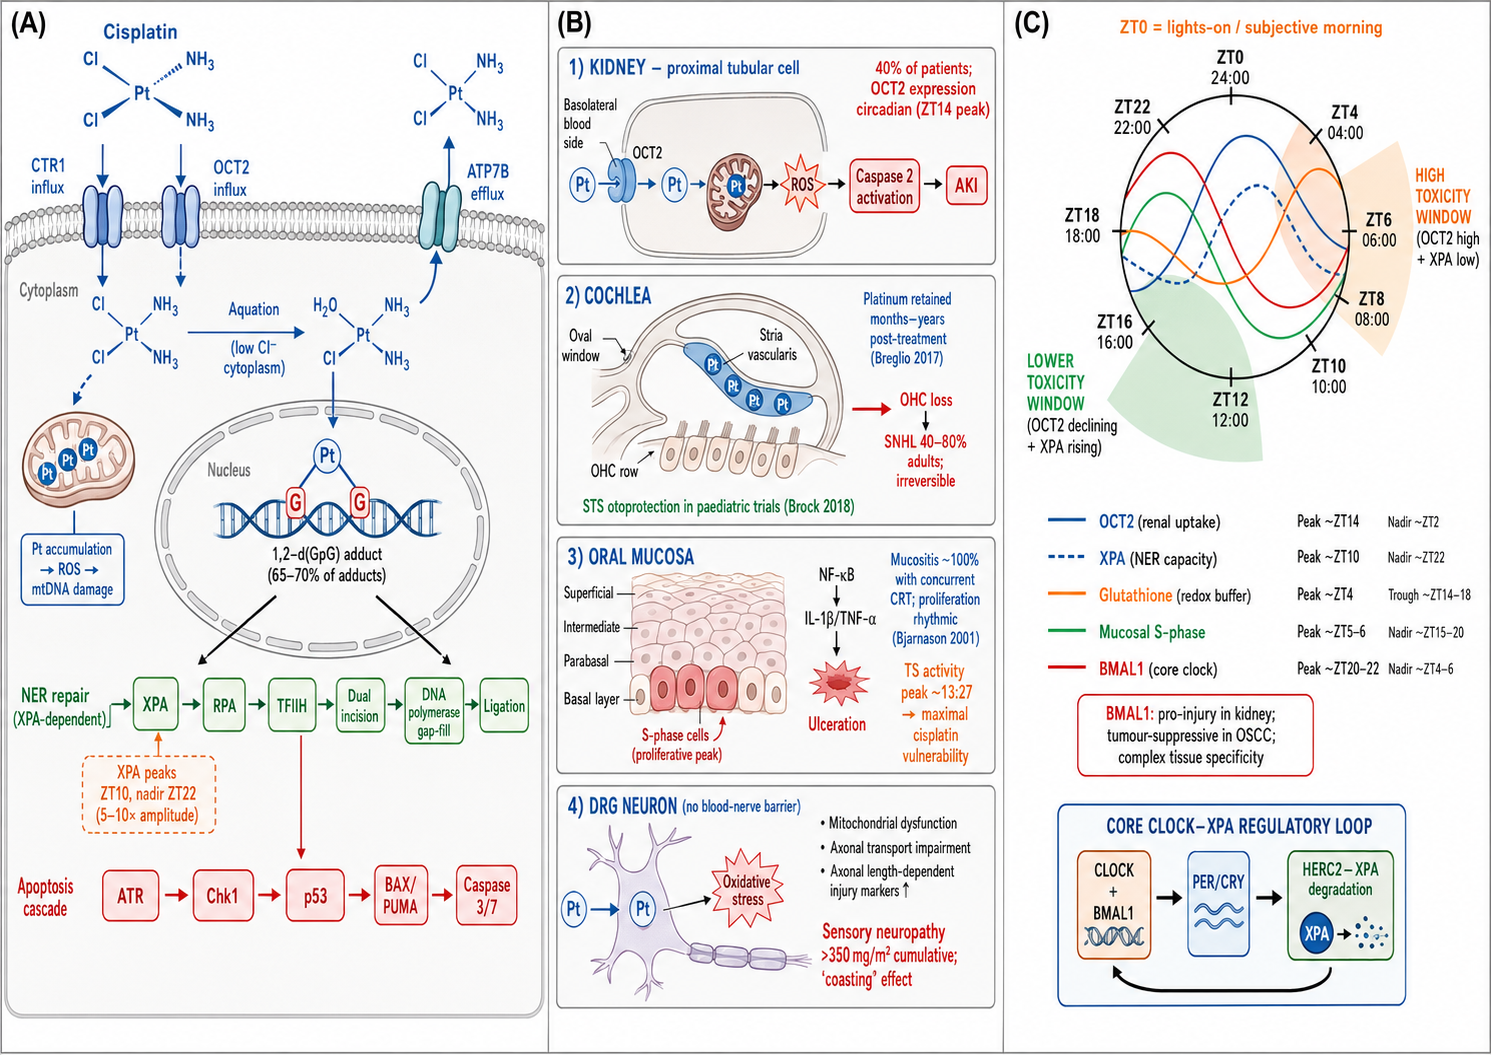
\includegraphics[width=\textwidth]{../figure/fig1}
  \captionof{figure}{\textbf{Cisplatin mechanism of action, organ-specific
    toxicity pathways, and circadian timing gates.}}
  \label{fig:mechanism}
\end{center}

{\footnotesize
\noindent\textbf{Figure~\ref{fig:mechanism} legend.}
    \textbf{(A)}~Cellular mechanism of cisplatin cytotoxicity. Cisplatin
    enters cells via CTR1 (influx) and OCT2 (tissue-specific influx in
    kidney and cochlea); intracellular export is mediated by ATP7B.
    Aquation in the low-chloride cytoplasm generates reactive platinum
    species that form 1,2-d(GpG) intrastrand crosslinks (65--70\% of
    adducts) on nuclear DNA. The NER pathway (XPA scaffold--RPA--TFIIH\allowbreak--
    dual incision--gap-fill ligation) resolves adducts when repair capacity
    is sufficient; when overwhelmed, ATR--Chk1--p53--BAX/PUMA--caspase~3/7
    apoptosis is activated. XPA protein abundance oscillates with circadian
    periodicity (peak ZT10, nadir ZT22; 5--10$\times$ amplitude), annotated
    by the dashed clock box.
    \textbf{(B)}~Organ-specific toxicity compartments. \emph{Kidney:}
    basolateral OCT2 concentrates cisplatin in proximal tubular S3 cells;
    ROS generation and caspase~2 activation drive AKI ($\sim$40\% of
    patients; OCT2 expression is circadian, peaking ZT14).
    \emph{Cochlea:} platinum is retained in stria vascularis and outer
    hair cells for months to years post-treatment~\cite{Breglio2017};
    irreversible SNHL affects 40--80\% of adults; STS otoprotection shown
    in paediatric trials~\cite{Brock2018}.
    \emph{Oral mucosa:} radiation and cisplatin synergise to activate
    NF-$\kappa$B--IL-1$\beta$/TNF-$\alpha$, driving ulceration in nearly
    all CRT patients; thymidylate synthase (TS) activity peaks at
    $\sim$13:27, identifying the mid-afternoon proliferative
    window~\cite{Bjarnason2001}.
    \emph{DRG neuron:} platinum accumulates without blood--nerve barrier
    protection; sensory neuropathy emerges above $\sim$350\,mg\,m$^{-2}$
    cumulative with a characteristic ``coasting'' effect~\cite{Park2013}.
    \textbf{(C)}~Circadian clock gates superimposed on a 24-hour dial
    (ZT0~=~lights-on/subjective morning). Five oscillating traces are
    shown: OCT2 renal uptake (solid blue; peak ZT14), XPA NER capacity
    (dashed blue; peak ZT10), glutathione redox buffer (green; trough
    resting phase), mucosal S-phase proliferation (orange; peak ZT5--6),
    and BMAL1 mRNA (red; peak early subjective night). Amber shading
    marks the \emph{high-toxicity window} (ZT6--8: rising OCT2, low XPA);
    teal shading marks the \emph{lower-toxicity window} (ZT14--20: declining
    OCT2, rising XPA). Inset: CLOCK/BMAL1--PER/CRY--HERC2-XPA degradation
    feedback loop. BMAL1 annotation reflects tissue-specific duality
    (Section~\ref{sec:gates}).
    Abbreviations: AKI, acute kidney injury; CTR1, copper transporter~1;
    DRG, dorsal root ganglion; NER, nucleotide excision repair; OHC,
    outer hair cell; OCT2, organic cation transporter~2; ROS, reactive
    oxygen species; SNHL, sensorineural hearing loss; STS, sodium
    thiosulfate; TS, thymidylate synthase; XPA, xeroderma pigmentosum
    complementation group~A; ZT, Zeitgeber time.\par}

\clearpage
\begin{center}
  \centering
  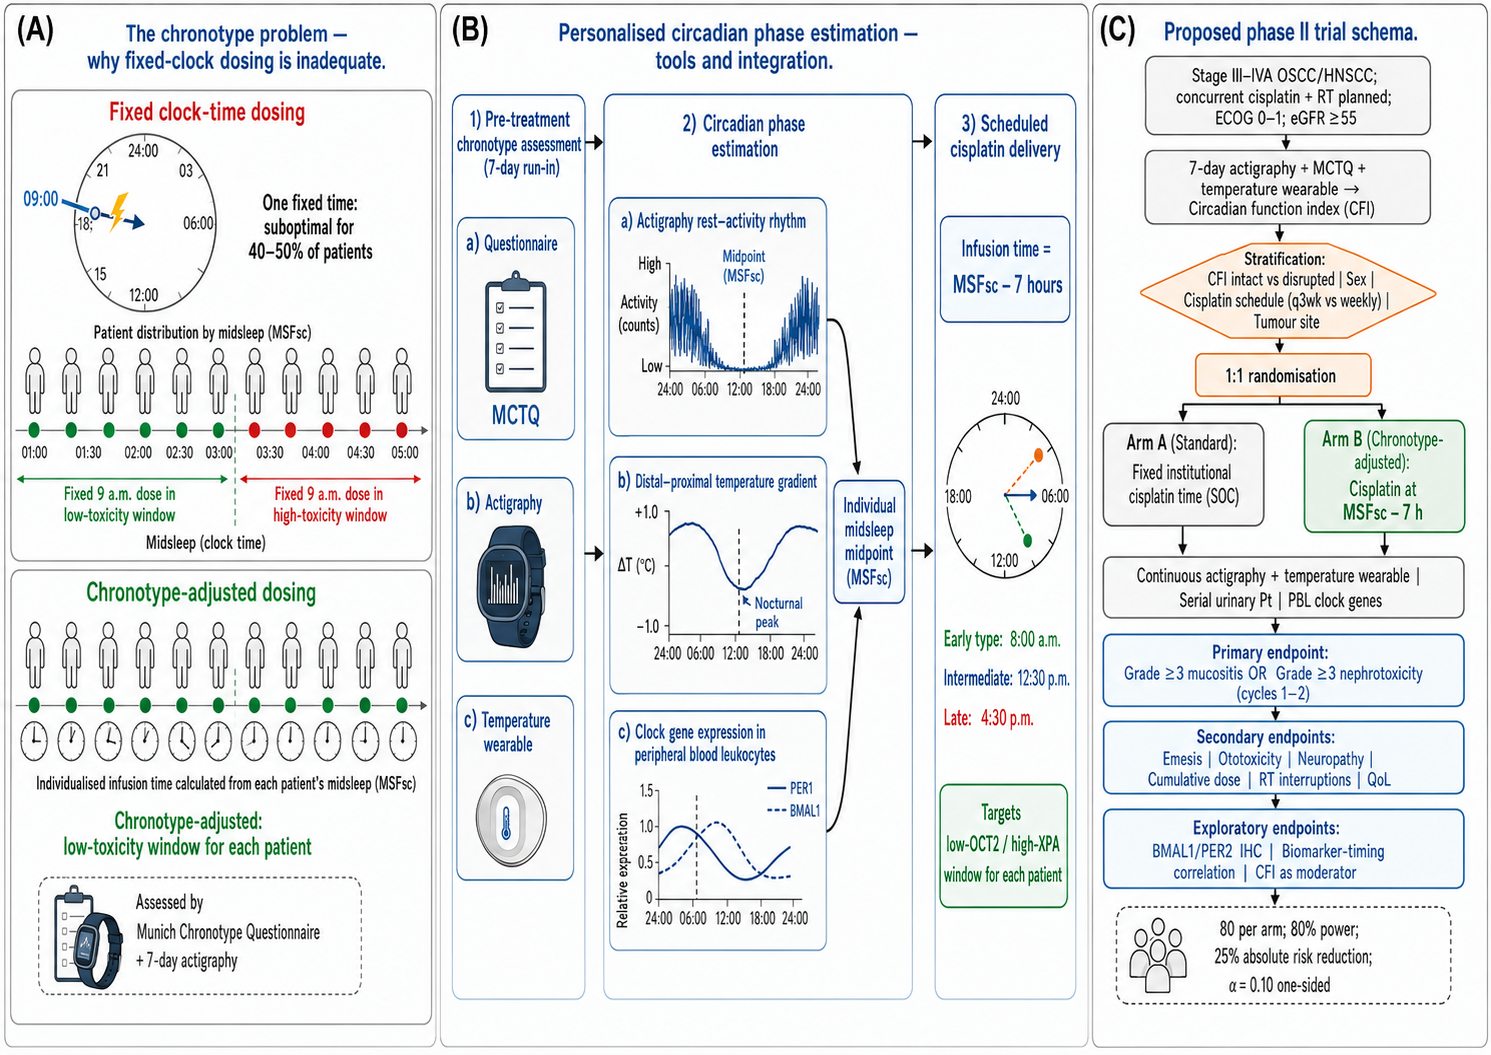
\includegraphics[width=\textwidth]{../figure/fig2}
  \captionof{figure}{\textbf{Proposed framework for chronotype-aware
    cisplatin scheduling in OSCC/HNSCC: rationale, phase estimation,
    and trial design.}}
  \label{fig:framework}
\end{center}

{\footnotesize
\noindent\textbf{Figure~\ref{fig:framework} legend.}
    \textbf{(A)}~The chronotype problem. \emph{Upper left:} Under fixed
    institutional clock-time dosing (e.g., 09:00), one single infusion
    time is applied to all patients regardless of their individual
    circadian phase. Patient icons are distributed by midsleep on free
    days (MSFsc; x-axis): early chronotypes (green; midsleep 01:00--02:30)
    receive cisplatin in their low-toxicity window, whereas late
    chronotypes (red; midsleep 03:30--05:00) receive it during their
    high-toxicity window --- suboptimal for 40--50\% of patients.
    \emph{Lower left:} Chronotype-adjusted dosing individualises the
    infusion time so that every patient receives cisplatin in their
    personal low-toxicity window, assessed by the Munich Chronotype
    Questionnaire (MCTQ) and 7-day actigraphy.
    \textbf{(B)}~Personalised circadian phase estimation. Three
    measurement streams converge to estimate individual midsleep (MSFsc):
    (a)~self-reported MCTQ; (b)~wrist actigraphy rest--activity rhythm
    (midpoint of inactivity marked); and (c)~continuous distal--proximal
    skin temperature gradient (nocturnal peak used as phase anchor), plus
    timed peripheral blood leukocyte (PBL) clock gene expression
    (PER1/BMAL1 at three time-points). The estimated MSFsc determines the
    infusion time via the formula \emph{Infusion time = MSFsc $-$ 7\,h},
    which targets the low-OCT2/high-XPA window for each
    patient~\cite{Oda2014, Kang2010}. Worked examples: early chronotype
    08:00; intermediate chronotype 12:30; late chronotype 16:30--17:00.
    \textbf{(C)}~Proposed phase~II randomised trial schema
    (Section~\ref{sec:future}). Eligible OSCC/HNSCC patients (stage
    III--IVA; concurrent cisplatin + RT; ECOG 0--1; CrCl~$\geq$~55;
    baseline audiogram) enter a 7-day actigraphy + MCTQ + temperature
    wearable run-in to estimate circadian function index (CFI). Patients
    are stratified by CFI (intact/disrupted), sex, cisplatin schedule
    (q3wk/weekly), and tumour site, then randomised 1:1 to Arm~A
    (standard fixed institutional time) or Arm~B (chronotype-adjusted:
    MSFsc~$-$~7\,h). Continuous actigraphy, temperature wearable, serial
    urinary platinum excretion, and PBL clock genes are collected
    throughout treatment. Primary endpoint: Grade~$\geq$3 mucositis or
    Grade~$\geq$3 nephrotoxicity within 6~weeks of first cisplatin
    (CTCAE~v5.0). Secondary endpoints: emesis, ototoxicity, neuropathy,
    cumulative cisplatin dose, RT interruptions, QoL (EORTC~QLQ-C30/
    H\&N35). Exploratory: BMAL1/PER2~IHC, biomarker-timing correlation,
    CFI as moderator. Sample size: 80/arm (80\% power, primary design
    target ARR~20\%, $\alpha$~=~0.10 one-sided).
    Abbreviations: CFI, circadian function index; CrCl, creatinine
    clearance; CTCAE, Common Terminology Criteria for Adverse Events;
    MCTQ, Munich Chronotype Questionnaire; MSFsc, midsleep on free days
    (sleep-corrected); OCT2, organic cation transporter~2; PBL, peripheral
    blood leukocytes; QoL, quality of life; RT, radiotherapy; XPA,
    xeroderma pigmentosum complementation group~A.\par}

\clearpage

%%
%% ================================================================
%% REFERENCES
%% ================================================================
%%
\bibliographystyle{elsarticle-num}
\bibliography{references}

\end{document}
